\chapter{\protect Results and Discussions}
\label{results}
According to the New Horizons team \cite{grundy2016formation}, CH$_4$ from Pluto may accumulate onto the surface of Charon by cold-trapping. The amount of CH$_4$ varies along the surface of Charon because it depends on the length of time the temperature is below 25 K which in turns depends on diurnal motion and thermal inertia of Charon. With an axis tilted by 112 degrees from the ecliptic, higher concentration of CH$_4$ will be accumulated at the pole (see chapter \ref{introduction} for details). In this chapter, we will investigate the following mainly by infrared spectroscopy: 1. The photoproducts produced by different concentration ratios of methane to ammonia, 2.the reaction mechanisms of each main products, 3. the photo products produced by EUV and VUV photons and 4. the functional groups of tholin formed by irradiation of VUV, EUV on different relative proportions of CH$_4$:NH$_3$ ice mixtures (the result is compared with the residues on Titan produced by Imanaka et al. \cite{imanaka2004laboratory}).

\section{The infrared spectra and peaks identification}
\begin{figure}
\centering
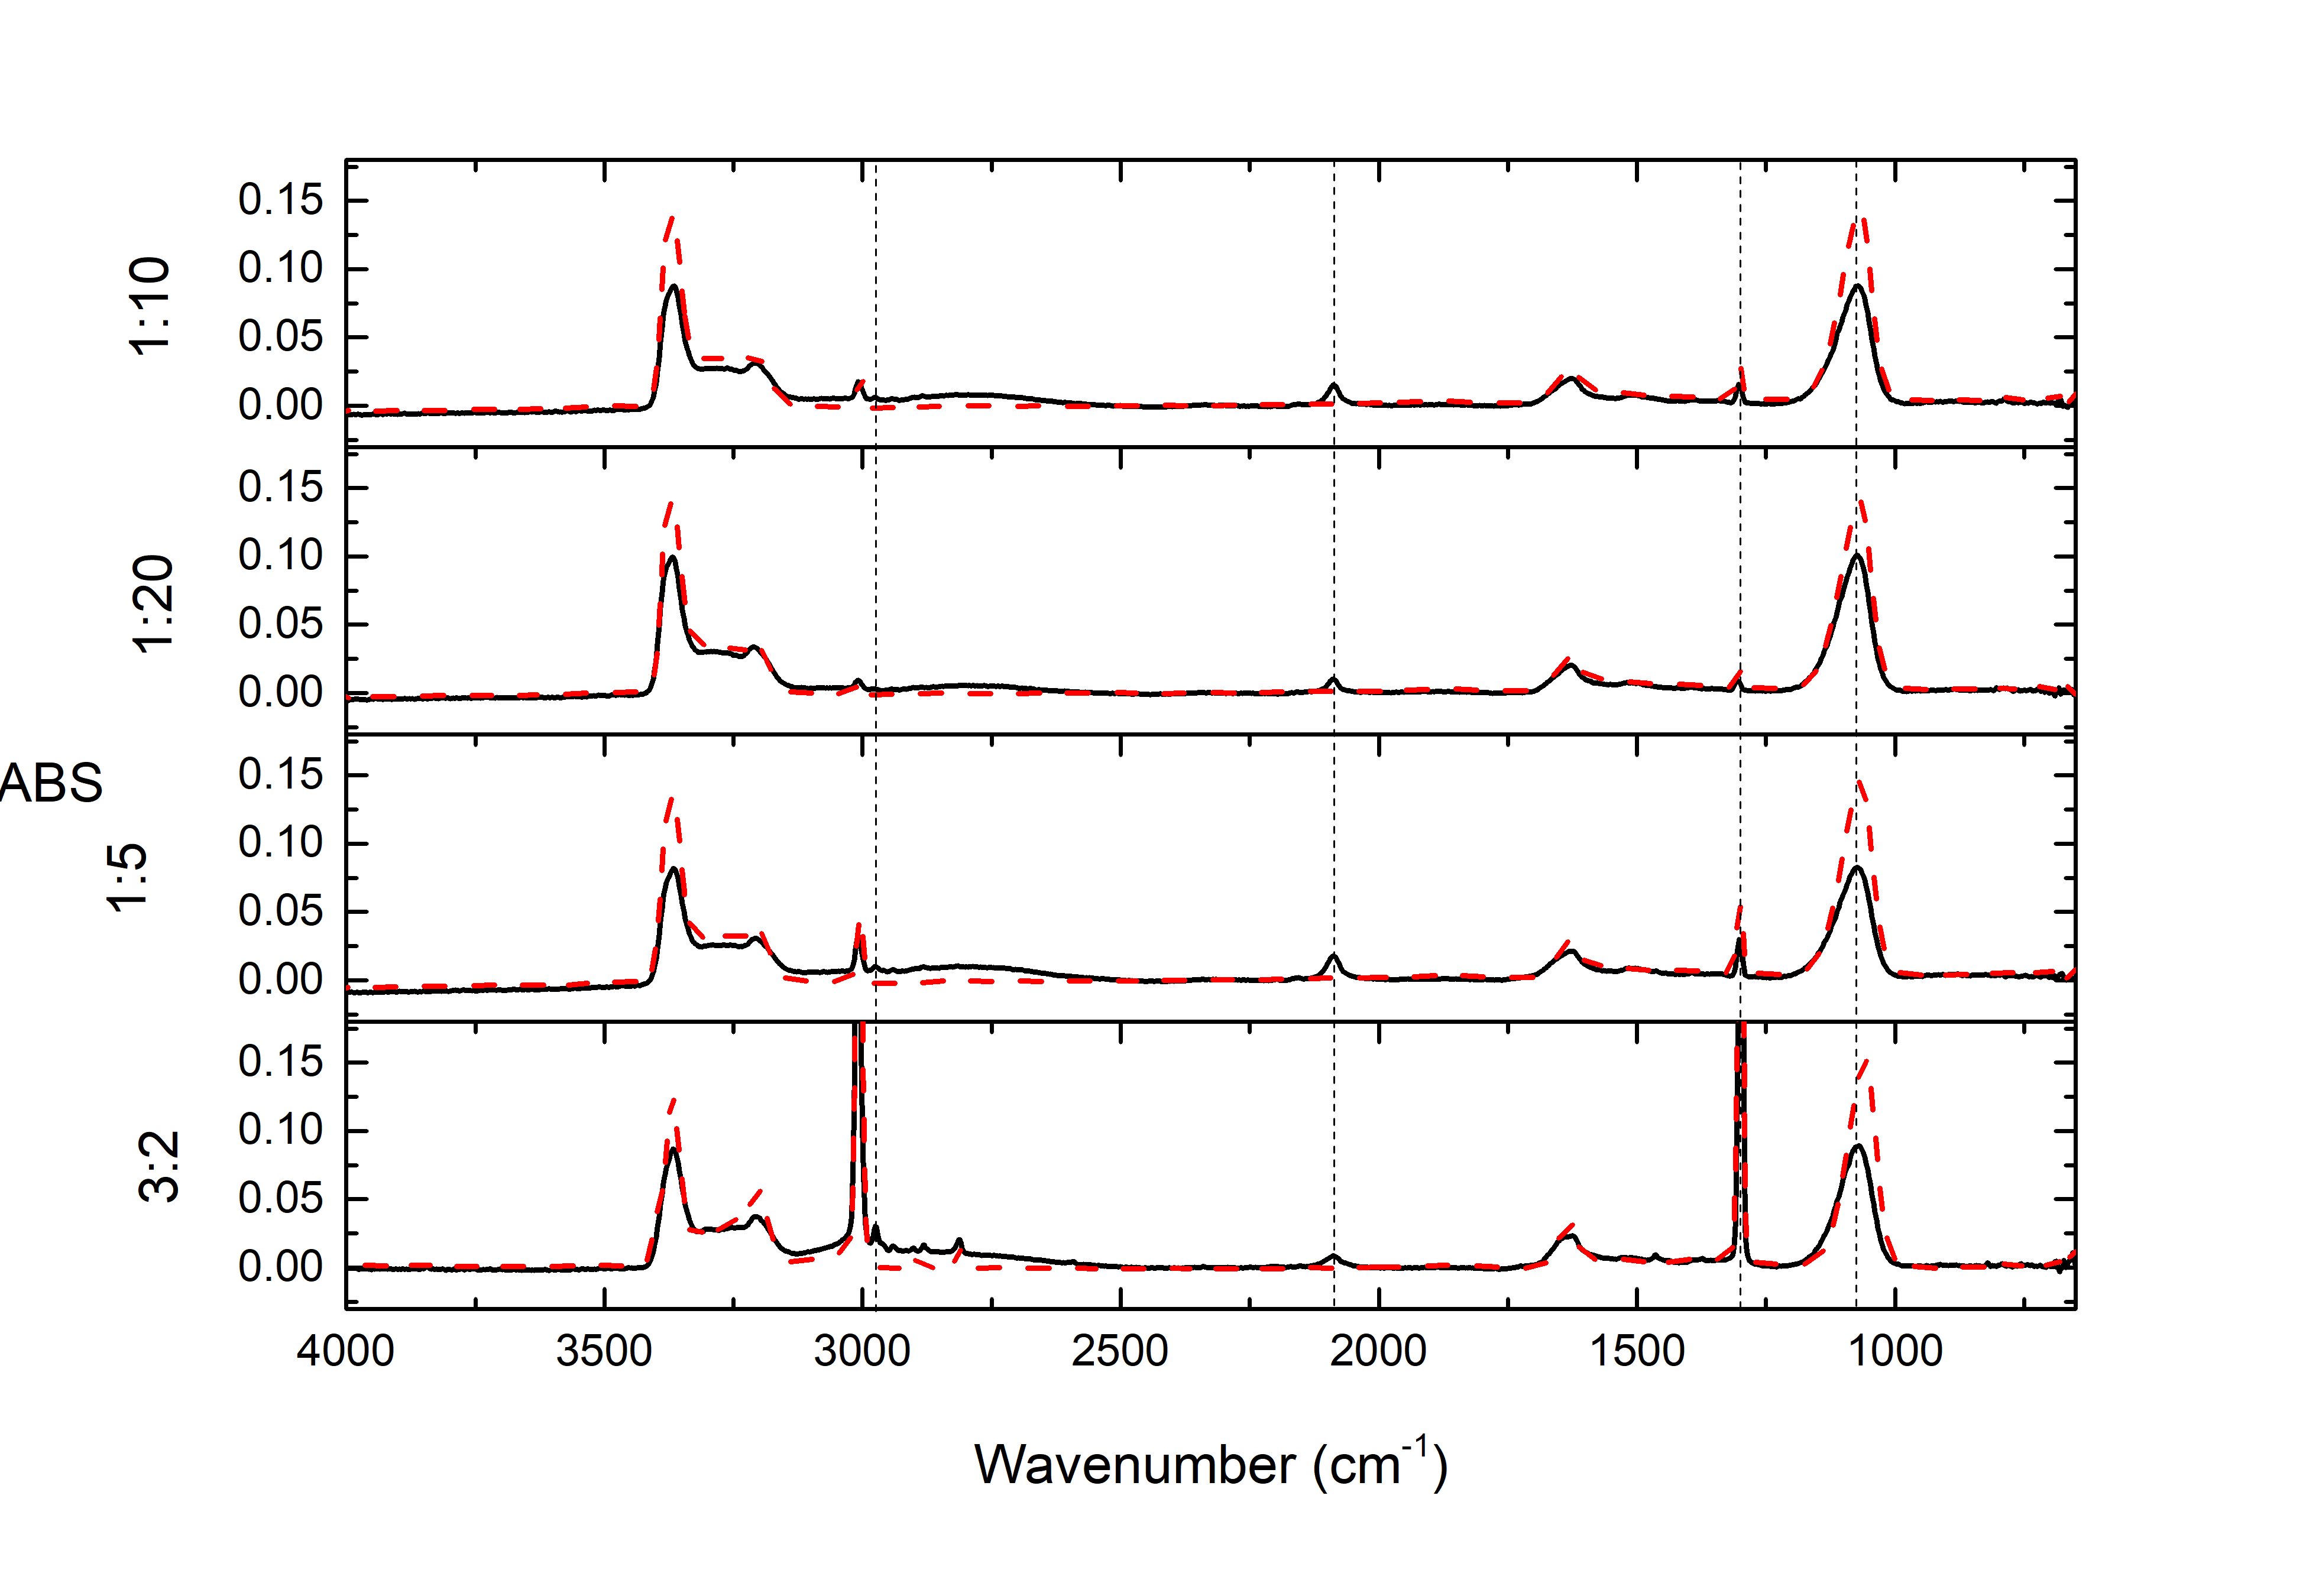
\includegraphics[width=\textwidth]{figures/chapter3/widerange.png}
\caption{The the infrared spectrum of CH$_4$ + NH$_3$ ice mixtures before irradiation (black) and VUV irradiated ice mixtures provided by MDHL. }
\label{fig:widerange}
\end{figure}

Figure \ref{fig:widerange} is a typical infrared spectrum of CH$_4$:NH$_3$ ice mixtures in different concentration ratios: 1:20, 1:10, 1:5 and 3:2 where ammonia is fixed with a column density 6 $\times$ 10$^{17}$ molecules cm$^{-2}$. We scan the IR spectrum prior to the irradiation at 15 K (for details of methodology, please refer to section \ref{sec:Experimental_Protocol}).\\

\begin{table}[htbp]
\caption{The strength of absorbance adopted in this thesis measured in literatures of pure ice samples}
\label{tab:Absorbance}
\begin{tabular}{cccccc}
\hline
\hline
Wavenumber (cm$^{-1}$) & Assignment  & Vibration & FWHM & A value ($\times 10^{-17}$) & Reference \\
\hline
2976 &  C$_2$H$_6$ & -CH$_3$ & - & 1.05 & 2 \\
2960 & C$_3$H$_8$ & -CH$_2$- & - & 2.58 & 2 \\
2086 & CN$^-$ & CN & - & 1.8 & 3 \\
1297 & CH$_4$ & CH deformation & 8 & 0.61 & 1 \\
1070 & NH$_3$ & "umbrella mode" & 68 & 1.7 & 1 \\
\hline
\end{tabular}
Reference: 1. d'Hendecourt and Allamandola (1986)\cite{d1986time} 2. Moore and Hudson (1998)\cite{moore1998infrared} 3. Noble et al. (2013) \cite{noble2012thermal}
\end{table}

The peaks used in column density calculations (by equation \ref{eq:column_density}) are labelled by dotted lines in the graph (figure\ref{fig:widerange}). We are aware that IR absorption strengths can vary depending on its environment, which means it will be different when it is pure, when it is mixed with other ices, and will vary with the relative proportions between ice components. We are justified to use the same absorption strength throughout our discussion to estimate the column density of each species and how the absorption area changes with concentration ratios of ice mixtures and photon energy. The absorption strengths we adopted are stated in table \ref{tab:Absorbance} \\

\begin{figure}
\centering
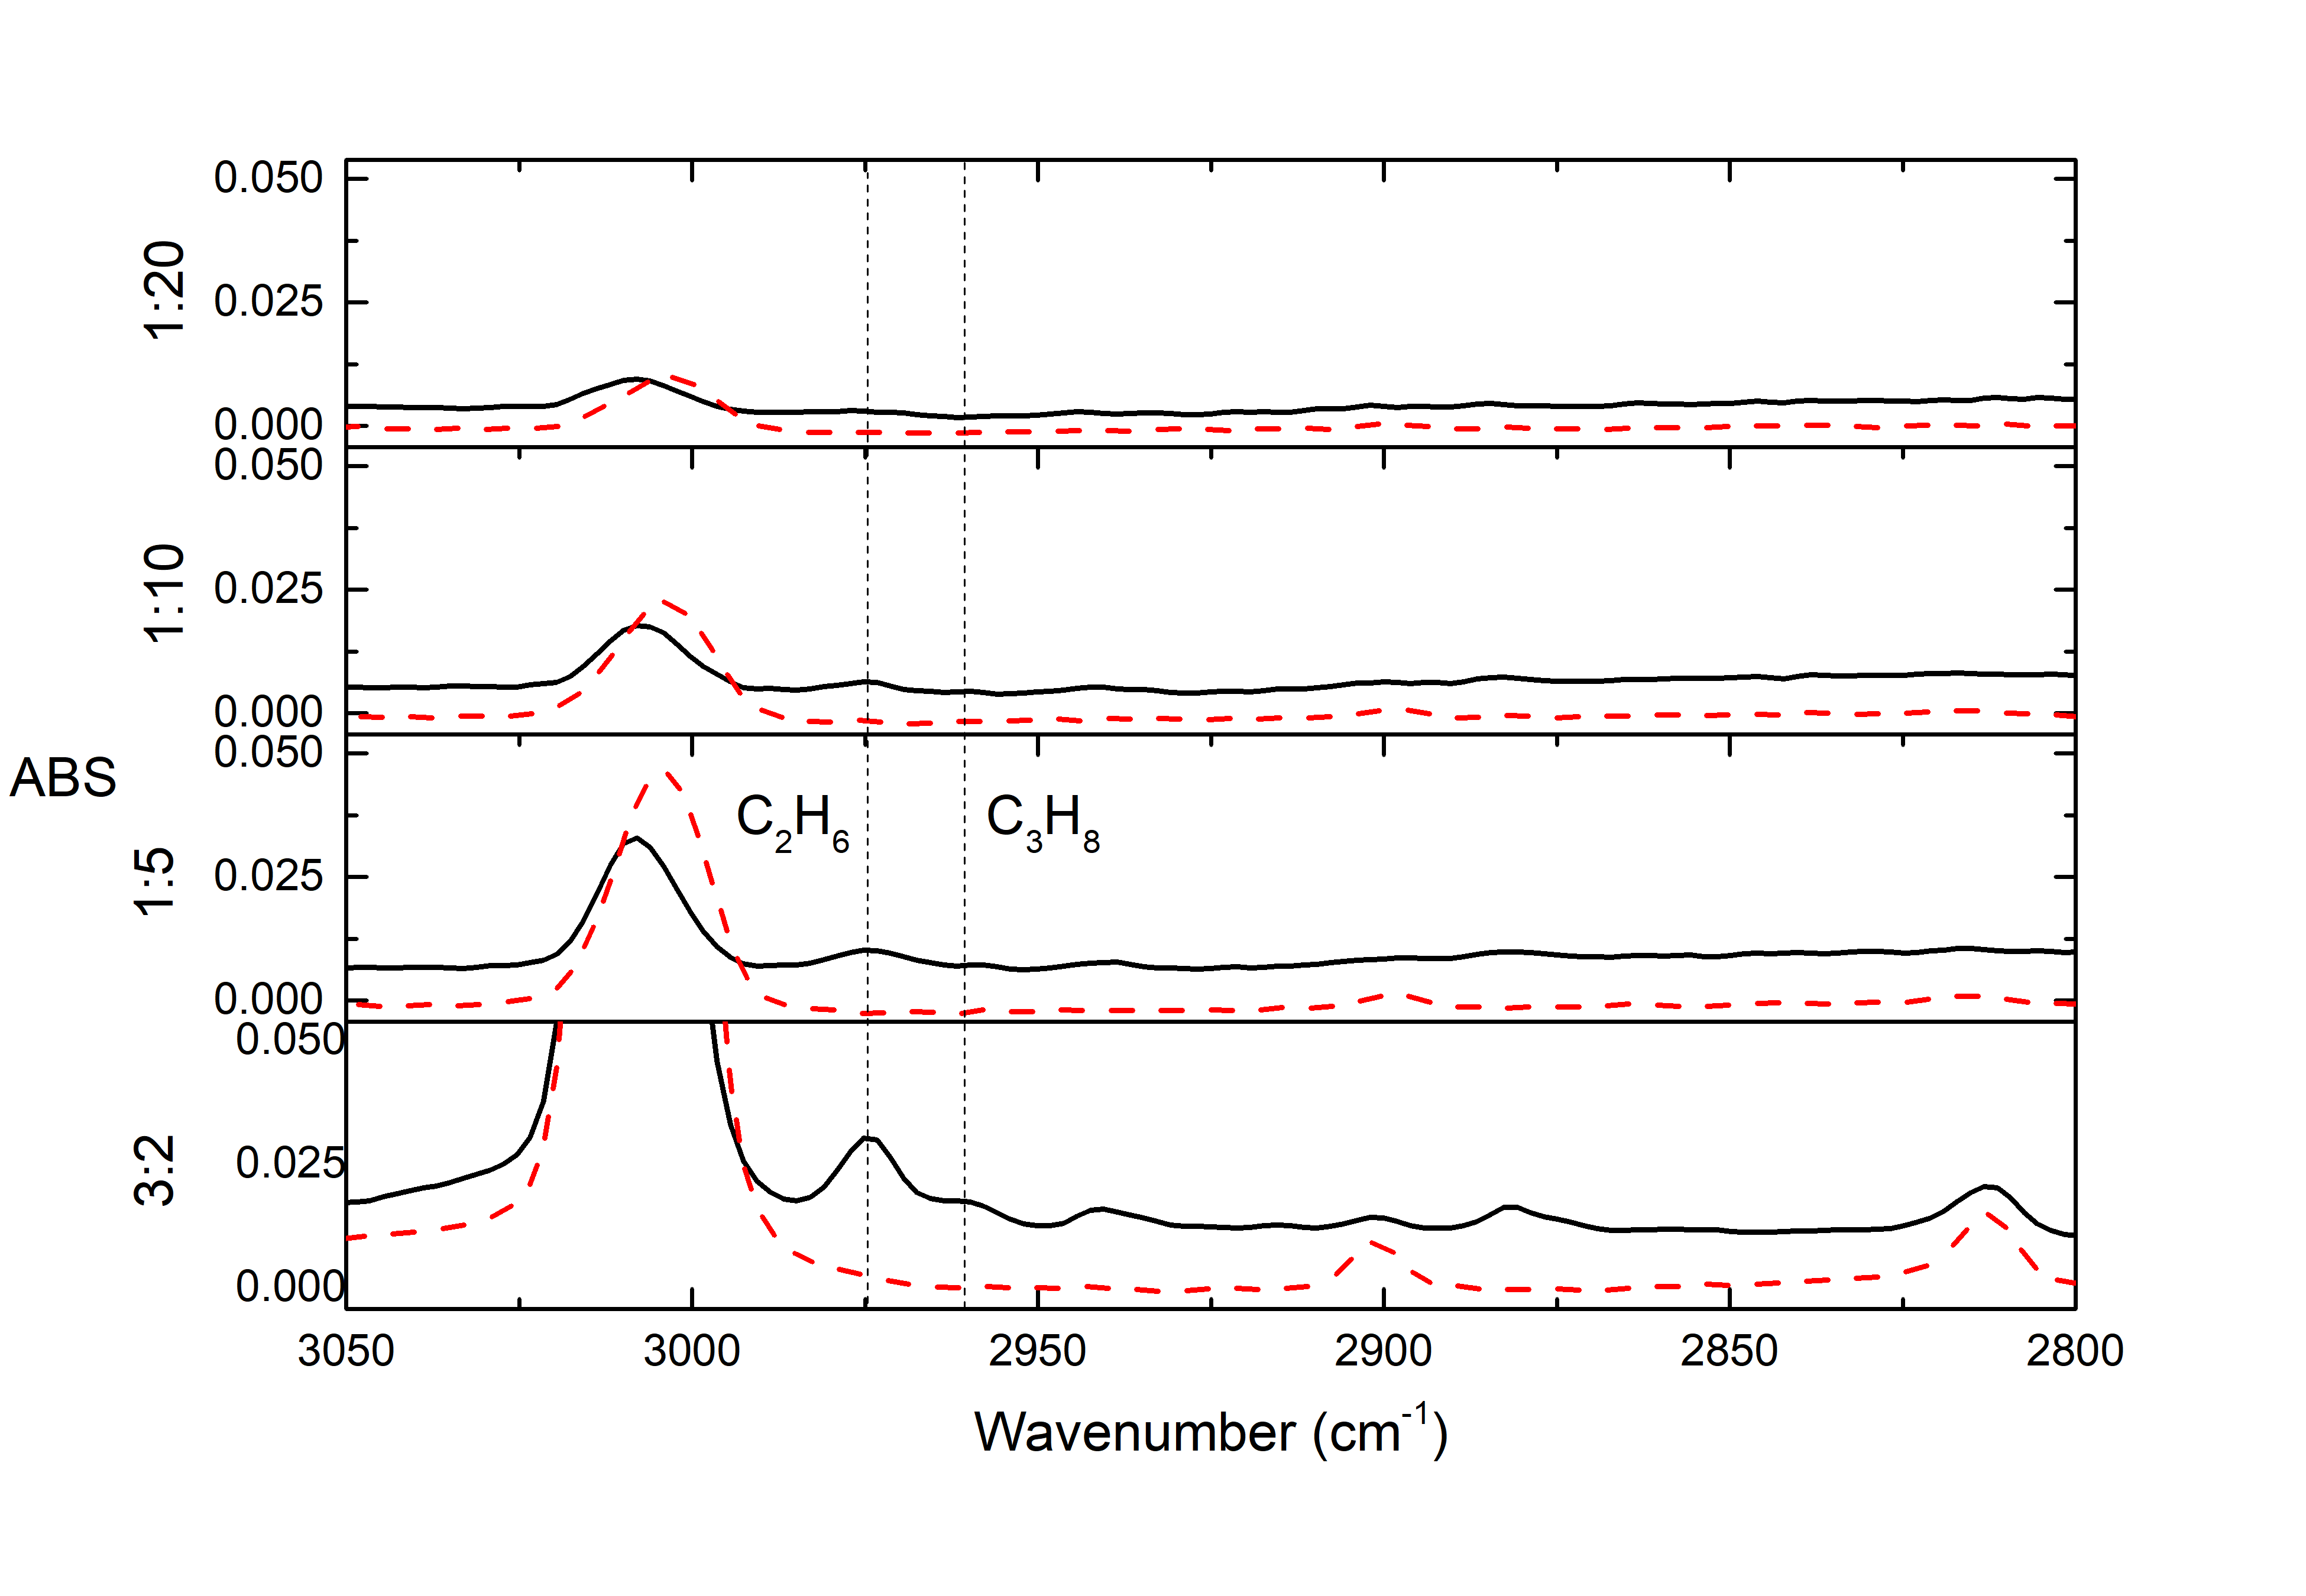
\includegraphics[width=\textwidth]{figures/chapter3/C2H6.png}
\caption{The the infrared spectrum of CH$_4$ + NH$_3$ ice mixtures of C$_2$H$_6$ and C$_3$H$_8$ before irradiation (black) and VUV irradiated ice mixtures provided by MDHL. }
\label{fig:C2H6}
\end{figure}

Figure \ref{fig:C2H6} is a zoomed view of figure \ref{fig:widerange}. Multiple peaks are used in product assignments, which are presented in table \ref{tab:WavenumberMDHL}. The absorption peak located at 2975 cm$^{-1}$ corresponds to the strongest vibration of C$_2$H$_6$. \\

The peak positioned at 2960 cm$^{-1}$ belongs to -CH$_2$- so we tentatively assign that as C$_3$H$_8$, which is the shortest carbon chain molecule contains -CH$_2$-. By fitting the peaks as a few gaussians, we deconvolute the overlapped C$_2$H$_6$ and C$_3$H$_8$ into two gaussians. The signal$-$to$-$noise ratio in CH$_4$:NH$_3$ = 1:10 is poor that we can not quantify the amount of C$_3$H$_8$ (figure \ref{fig:C2H6}).\\

\begin{figure}
\centering
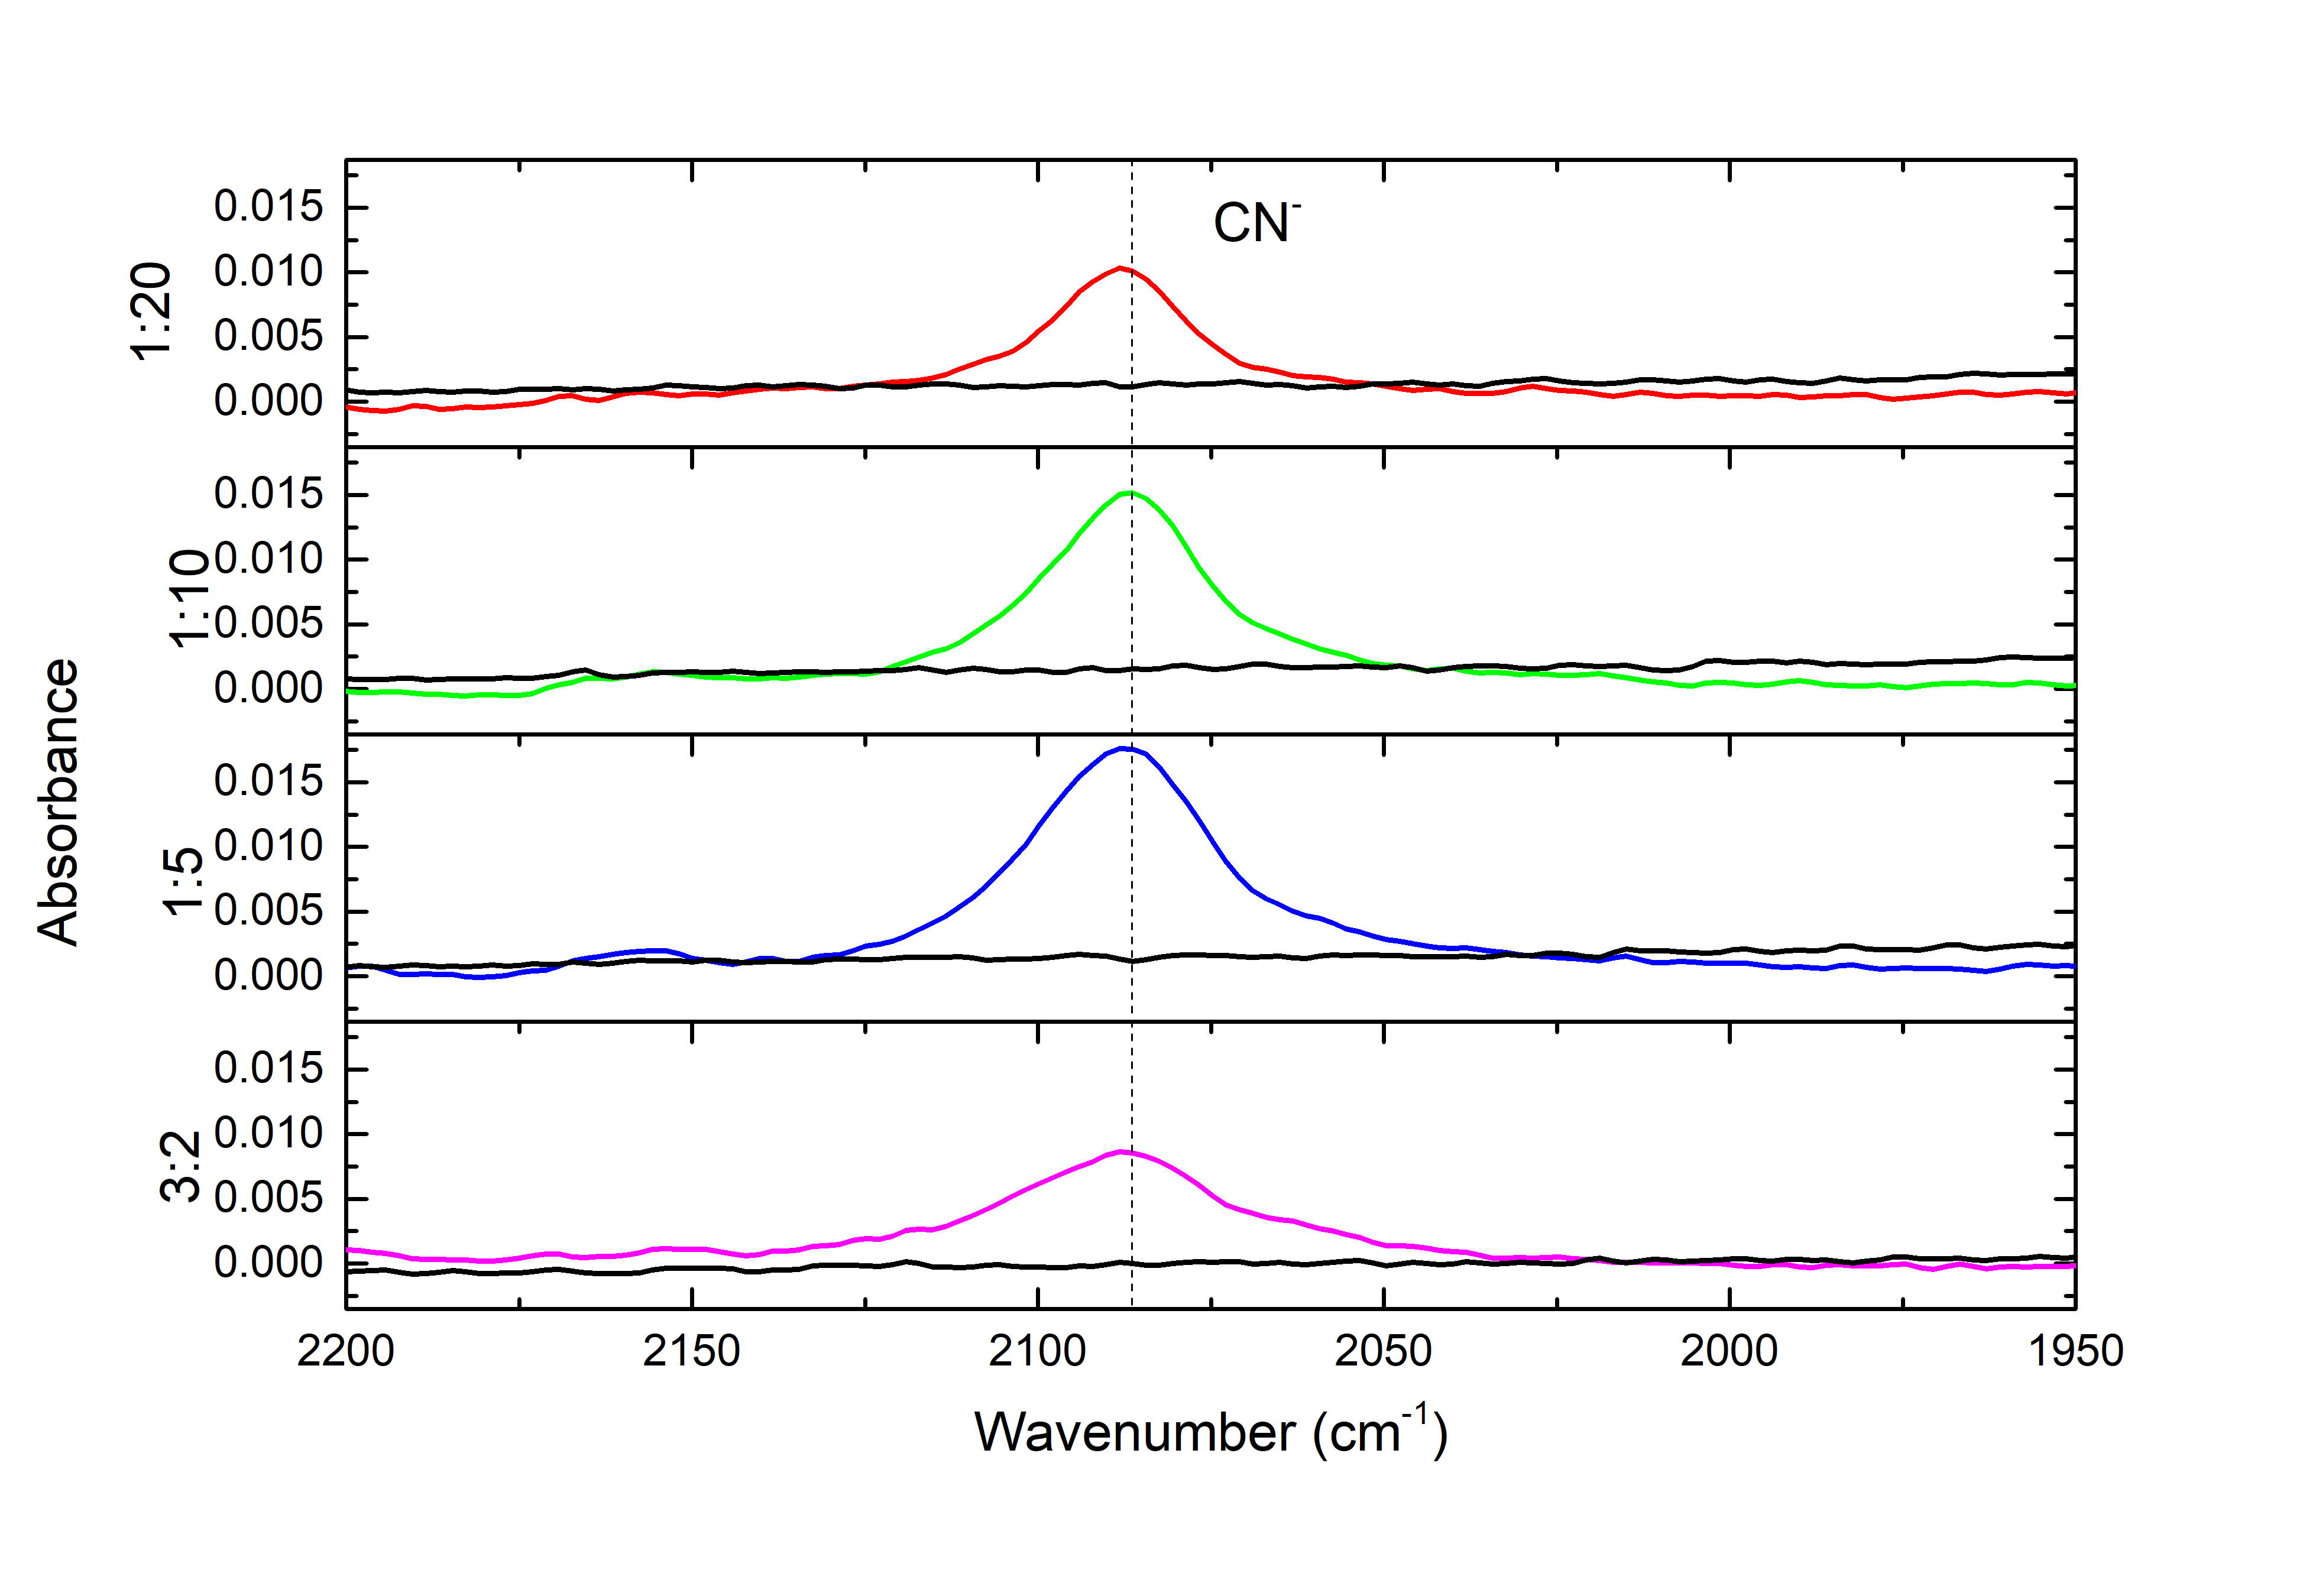
\includegraphics[width=\textwidth]{figures/chapter3/CN.png}
\caption{The infrared spectrum of CH$_4$ + NH$_3$ ice mixtures of C$_2$H$_6$ and C$_3$H$_8$ before irradiation (black) and VUV irradiated ice mixtures provided by MDHL. }
\label{fig:CN}
\end{figure}

Figure \ref{fig:CN} is a zoomed infrared absorption spectrum of CN$^-$. we assign the peak 2086 cm$^{-1}$ to CN$^-$  but not a combination of HCN and CN$^-$. The assignment is based on a absence in CN bending mode at 848 cm$^{-1}$. In the case CH$_4$ + NH$_3$ = 3:2, we may observe a peak located at 820 cm$^{-1}$, which is with a FWHM half of HCN and it is eliminated at 50 K during the warm-up phase. Since 50 K is the desorbing temperature of C$_2$H$_6$ and the peak position is close to $\nu$12 mode of C$_2$H$_6$, we believe that the 820 cm$^{-1}$ peak is contributed by C$_2$H$_6$. Therefore, we may assign our peak located at 2086 cm$^{-1}$ as purely CN$^-$. After identification of the main products (C$_2$H$_6$, CN$^-$ and C$_3$H$_8$), we will look into the mechanisms one by one in the next section.\\

\begin{table}[htbp]
\caption{The peak positions of identified substances after irradiation in different relative proportions of ice mixtures.}
\label{tab:WavenumberMDHL}
\begin{tabular}{ccccccc}
\hline
\hline
\multicolumn{2}{c}{Literture assignments} & \multicolumn{4}{c}{CH$_4$:NH$_3$ ratio (MDHL)} &  \\
\hline
Wavenumber & Identified IR modes & 1:5  & 1:10  & 1:20  & 3:2  & Ref. \\
(cm$^{-1}$) &   & (cm$^{-1}$) & (cm$^{-1}$) & (cm$^{-1}$) & (cm$^{-1}$) &\\
\hline
3375 & $\nu_3$ (NH$_3$) & 3366 & 3366 & 3369 & 3367 & 1 \\
3210 & $\nu_1$ (NH$_3$) & 3207 & 3208 & 3210 & 3205 & 1 \\
2972 & $\nu_{10}$ (C$_2$H$_6$) & 2975 & - & - & 2975 & 3 \\
2960 & C$_3$H$_8$ & - & - & - & 2960 & 7 \\
2941 & $\nu_8+\nu_11$ (C$_2$H$_6$) & 2940 & - & - & 2940 & 3 \\
2904 & $\nu_1$ (CH$_4$) & 2901 & - & - & 2901 & 5 \\
2879 & $\nu_5$ (C$_2$H$_6$) & 2882 & 2883 & - & 2882 & 3 \\
2814 & $\nu_2+\nu_4$ (CH$_4$) & - & - & - & 2815 & 5 \\
2083 & $\nu$ (CN$^-$) & 2088 & 2087 & 2088 & 2088 & 2 \\
1625 & $\nu_4$ (NH$_3$) & 1625 & 1625 & 1626 & 1631 & 1 \\
1514 & $\delta$ (NH$_2$) & 1509 & 1507 & 1505 & 1511 & 6 \\
1465-1440 & deform CH$_2$ scissor & 1461 & - & - & 1463 & 3,4 \\
1390-1370 & CH$_3$ sym deform & 1394 & 1394 & 1394 & 1372 & 4 \\
1298 & $\nu_4$ (CH$_4$) & 1301 & 1302 & 1305 & 1299 & 2 \\
1075 & $\nu_2$ (NH$_3$) & 1073 & 1072 & 1072 & 1072 & 1 \\
820 & $\nu_{12}$ (C$_2$H$_6$) & - & - & - & 820 & 3 \\
\hline
\end{tabular}\\
Reference: 1. Bossa et al. 2008 \cite{bossa2008carbamic} 2. Moore and Hudson 2003 \cite{moore2003infrared} 3. Kim et al. 2010 \cite{kim2010abiotic} 4. Socrates 2001 \cite{socrates2001infrared} 5. Bennet and Kaiser 2007 \cite{bennett2007formation} 6. Zheng et al. 2008 \cite{zheng2008formation} 7. Hudson and Moore 2004 \cite{hudson2004reactions}
\end{table}

\section{Reaction mechanisms and fitting results} %mechanisms
\subsection{C$_2$H$_6$}
The formation of C$_2$H$_6$ in astrophysical environment is mainly a combination with 2 CH$_3$ radicals \cite{bennett2006laboratory}:
\begin{equation}
CH_4 + hv \rightarrow CH_3
\label{eq:CH3}
\end{equation}
\begin{equation}
2 CH_3 \rightarrow C_2H_6
\label{eq:C2H6}
\end{equation}

The energy requires to break the CH bond of CH$_4$ is 4.42 eV. The recombination of 2 CH$_3$ radicals forms a internal excited C$_2$H$_6$, and releases 3.74 eV to the surrounding matrixs or proceeds further to become ethly radicals (C$_2$H$_5$) or ethene (C$_2$H$_4$) (required extra of 0.53 and 0.84 eV respectively. \cite{bennett2006laboratory}. Therefore, the process in equation \ref{eq:C2H6} is a no-barrier exothermic process. The formed C$_2$H$_6$ is internally excited that it is able to become C$_2$H$_4$ etc. Figure \ref{fig:lab_C2H6} depicts the formation column density as a function of irradiation time of C$_2$H$_6$ in different relative proportions of irradiated ice mixtures.  As the formation only depends on CH$_4$, we may use first order kinetics equation to fit the column density versus photon dose.\\

\begin{equation}
[C_2H_6] = [C_2H_6]_0(1 - e^{-kt})
\label{eq:1step}
\end{equation}

The fitting results are shown in table \ref{tab:fittingC2H6}. From table \ref{tab:fittingC2H6}, the production rate is nearly proportional to the initial CH$_4$ concentrations.  Note that C$_2$H$_6$ is not detected in CH$_4$ to NH$_3$ = 1:20 ice mixtures.\\

\begin{figure}
\centering
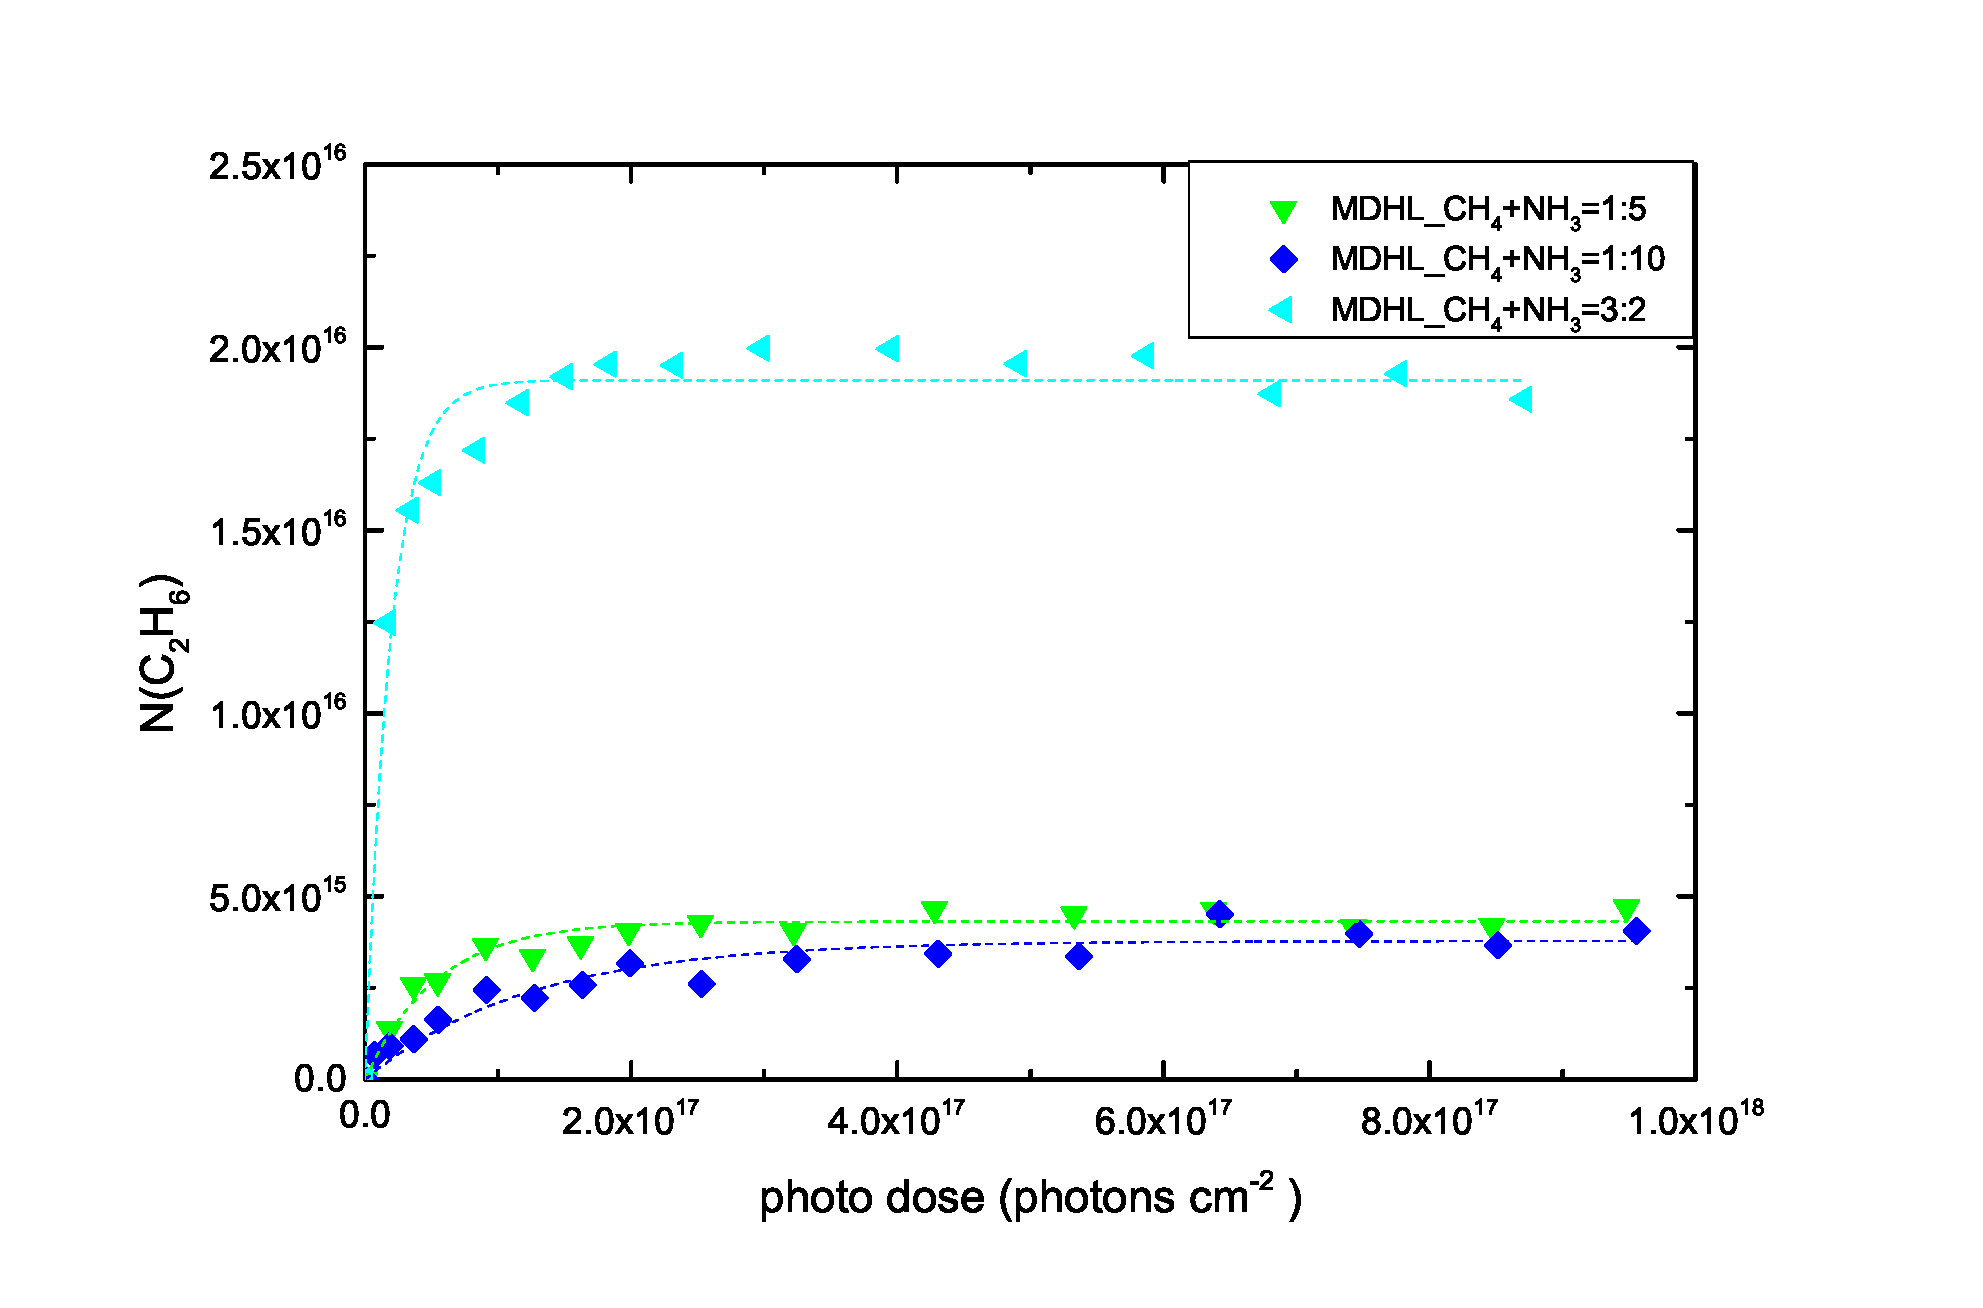
\includegraphics[width=\textwidth]{figures/chapter3/Lab_C2H6.eps}
\caption{The column density of C$_2$H$_6$ during CH$_4$ + NH$_3$ ice mixtures irradiated by MDHL. }
\label{fig:lab_C2H6}
\end{figure}

\begin{table}[htbp]
\caption{The fitting results of C$_2$H$_6$ by [C$_2$H$_6$]=[C$_2$H$_6$]$(1 - e^{-k_1 t})$}
\label{tab:fittingC2H6}
\begin{tabular}{ccc}
\hline
\hline
Ratio of CH$_4$:NH$_3$ & A (x10$^{15}$ molecules cm$^{-2}$) & k (x10$^{-17}$ photon$^{-1}$) \\
\hline
1:10 & 2.90 $\pm$ 1.25 & 0.92 $\pm$ 0.15 \\
1:5 & 4.16 $\pm$ 0.28 & 2.28 $\pm$ 0.28 \\
3:2 & 19.2 $\pm$ 0.15 & 5.28 $\pm$ 0.25 \\
\hline
\end{tabular}
\end{table}


\subsection{C$_3$H$_8$}

Propane is a secondary product formed by a combination of either C$_2$H$_6$ + CH$_2$ (equation \ref{eq:C3H81})or C$_2$H$_4$ + CH$_4$ (equation \ref{eq:C3H82}). From Bennet et al. (2006) \cite{bennett2006laboratory}, C$_2$H$_4$ is decomposed by the internally excited C$_2$H$_6$. With subsequently impinging electrons, it is degraded into C$_2$H$_3$ and C$_2$H$_2$ with an energy barrier of 4.69 and 4.06 eV respectively.
\begin{equation}
C_2H_6 + CH_2 \rightarrow C_3H_8
\label{eq:C3H81}
\end{equation}
\begin{equation}
C_2H_4 + CH_4 \rightarrow C_3H_8
\label{eq:C3H82}
\end{equation}

\begin{figure}
\centering
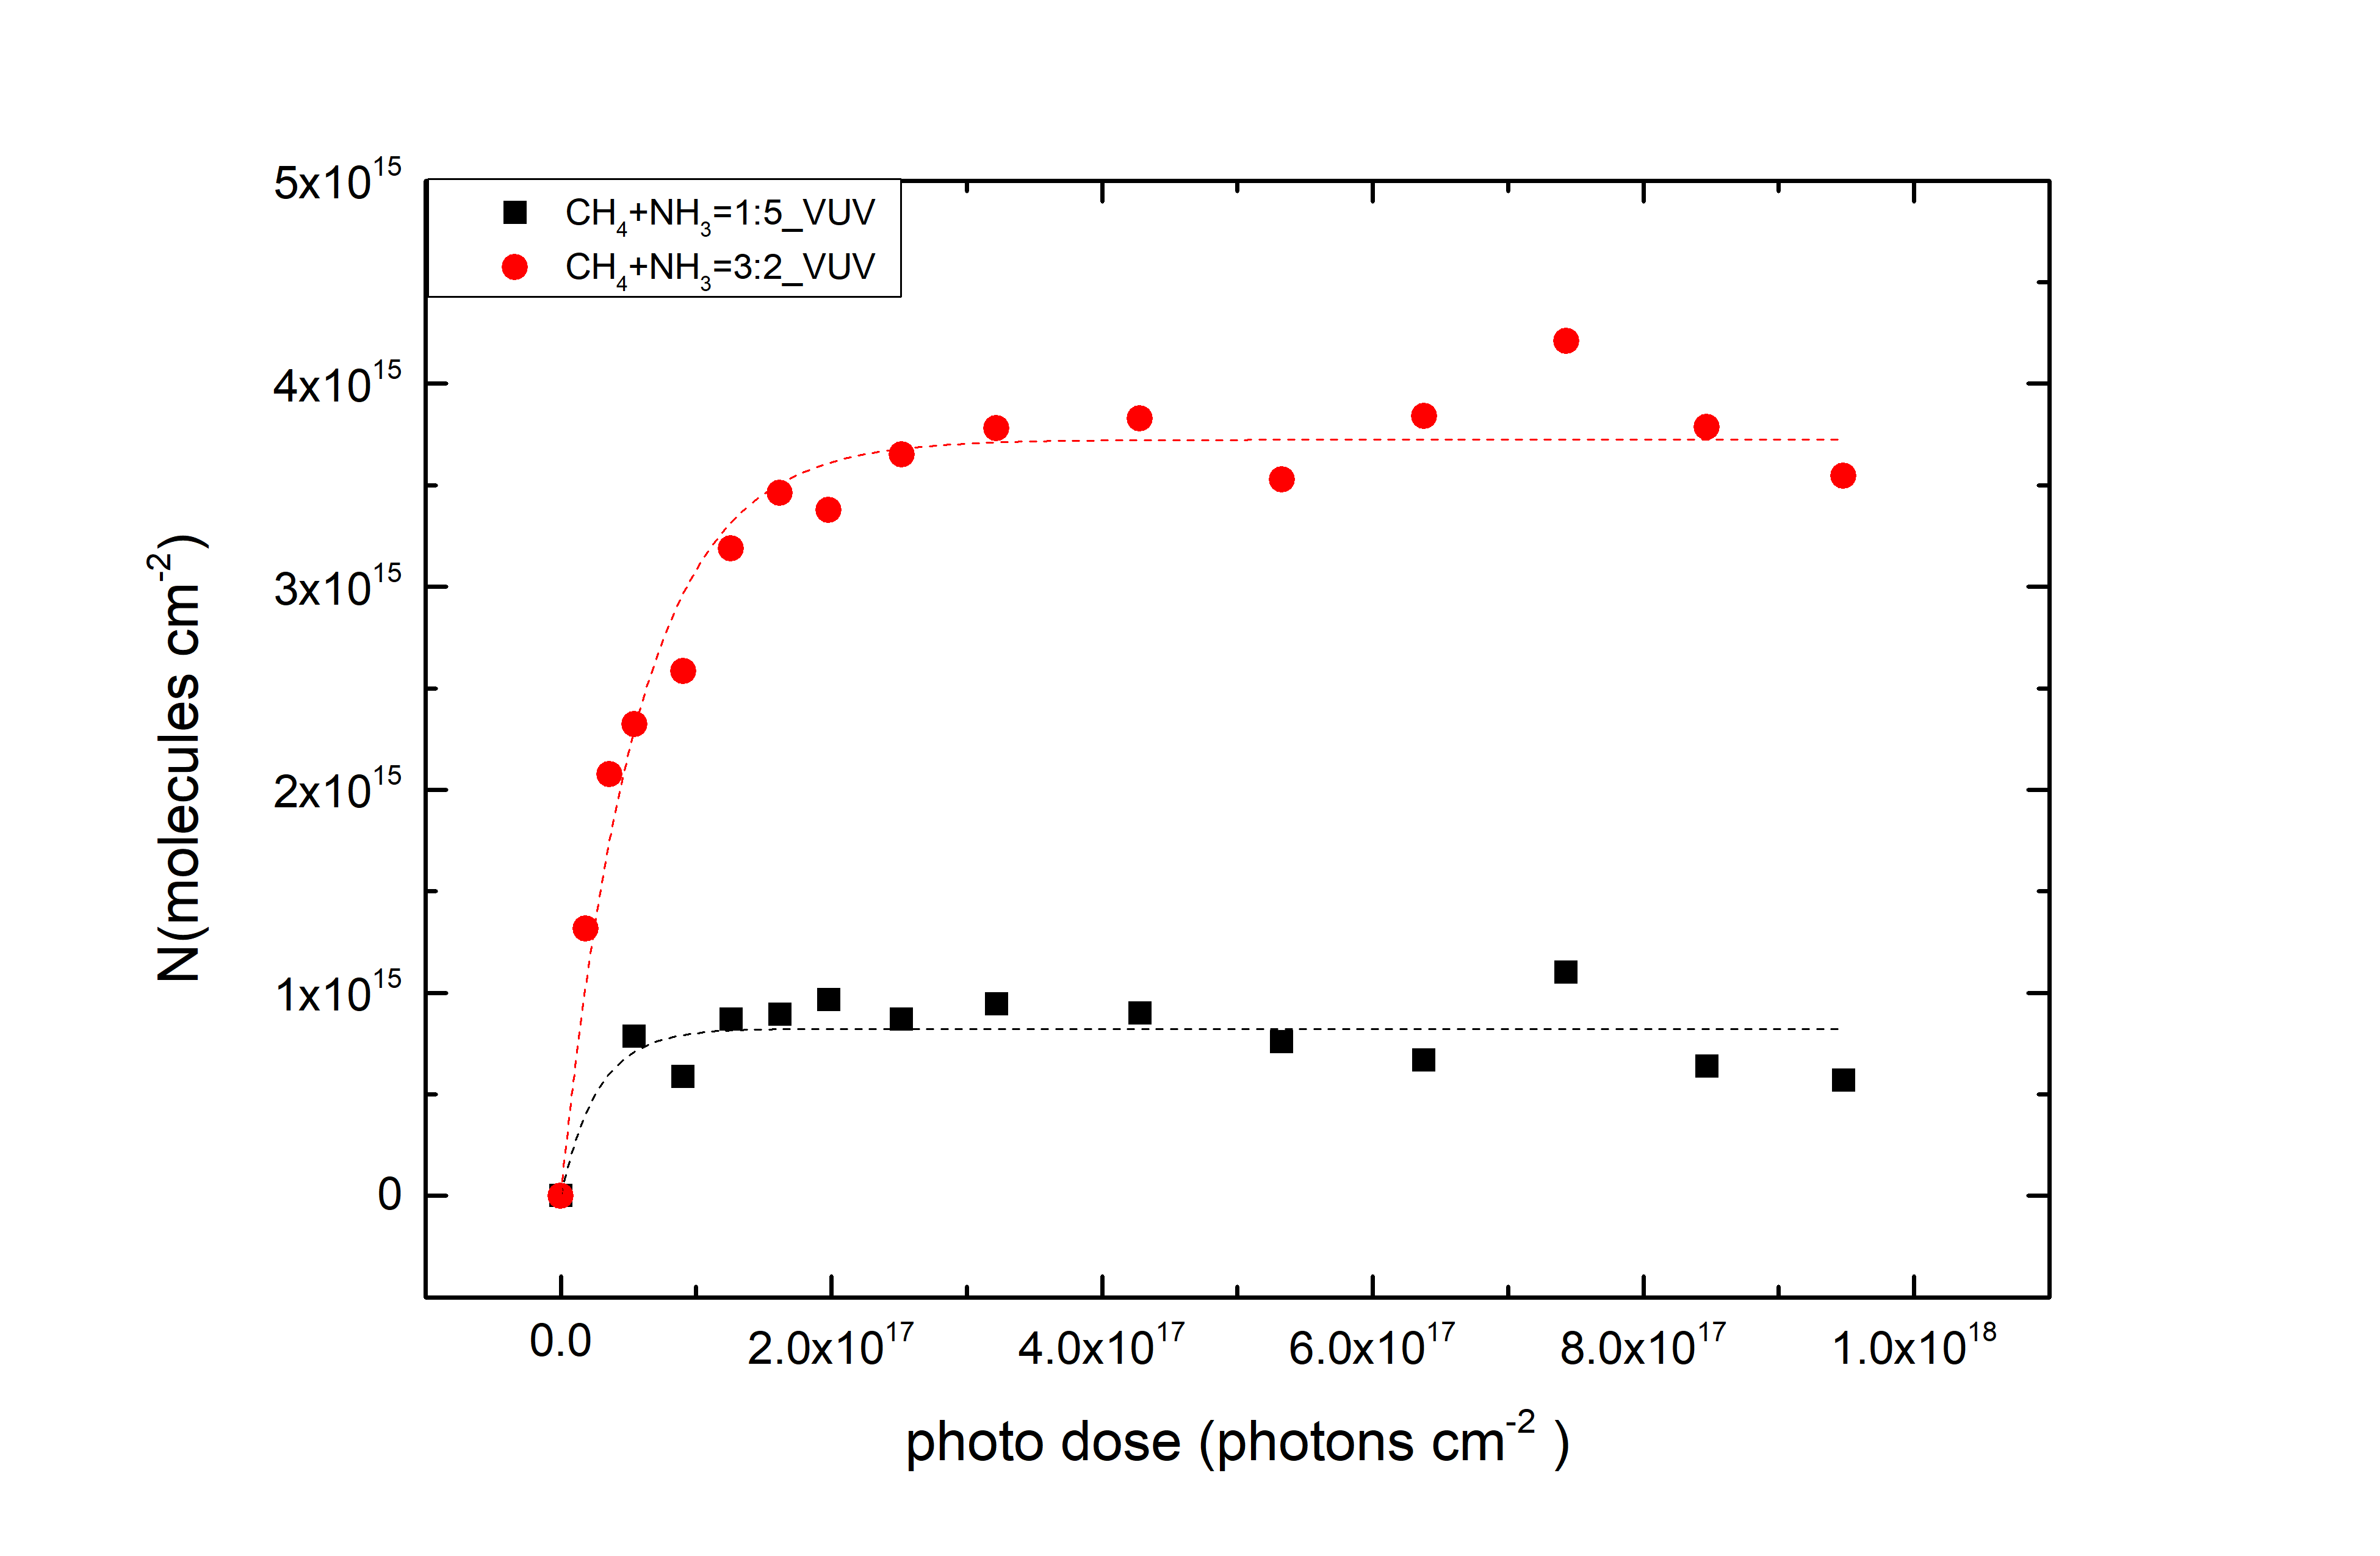
\includegraphics[width=\textwidth]{figures/chapter3/VUV_C3H8.png}
\caption{The column density of C$_3$H$_8$ during CH$_4$ + NH$_3$ ice mixtures irradiated by MDHL. }
\label{fig:lab_C3H8}
\end{figure}

\begin{table}[htbp]
\caption{The fitting results of C$_3$H$_8$ by [C$_3$H$_8$]=[C$_3$H$_8$]$(1 - e^{-k_1 t})$}
\label{tab:fittingC3H8}
\begin{tabular}{ccc}
\hline
\hline
Ratio of CH$_4$:NH$_3$ & A (x10$^{15}$ molecules cm$^{-2}$) & k (x10$^{-17}$ photon$^{-1}$) \\
\hline
1:5 & 0.46 $\pm$ 0.17 & 2.89 $\pm$ 2.44 \\
3:2 & 3.84 $\pm$ 0.18 & 2.08 $\pm$ 0.18 \\
\hline
\end{tabular}
\end{table}

The column densities are shown in figure \ref{fig:lab_C3H8}, where the fitting results are shown in table \ref{tab:fittingC3H8}. Since the C$_3$H$_8$ detection in CH$_4$ + NH$_3$ = 1:5 ice mixtures are close to our detection limits, the errors of the fitting results would attributes to a meaningless fitting.


\subsection{CN$^-$}

\begin{figure}
\centering
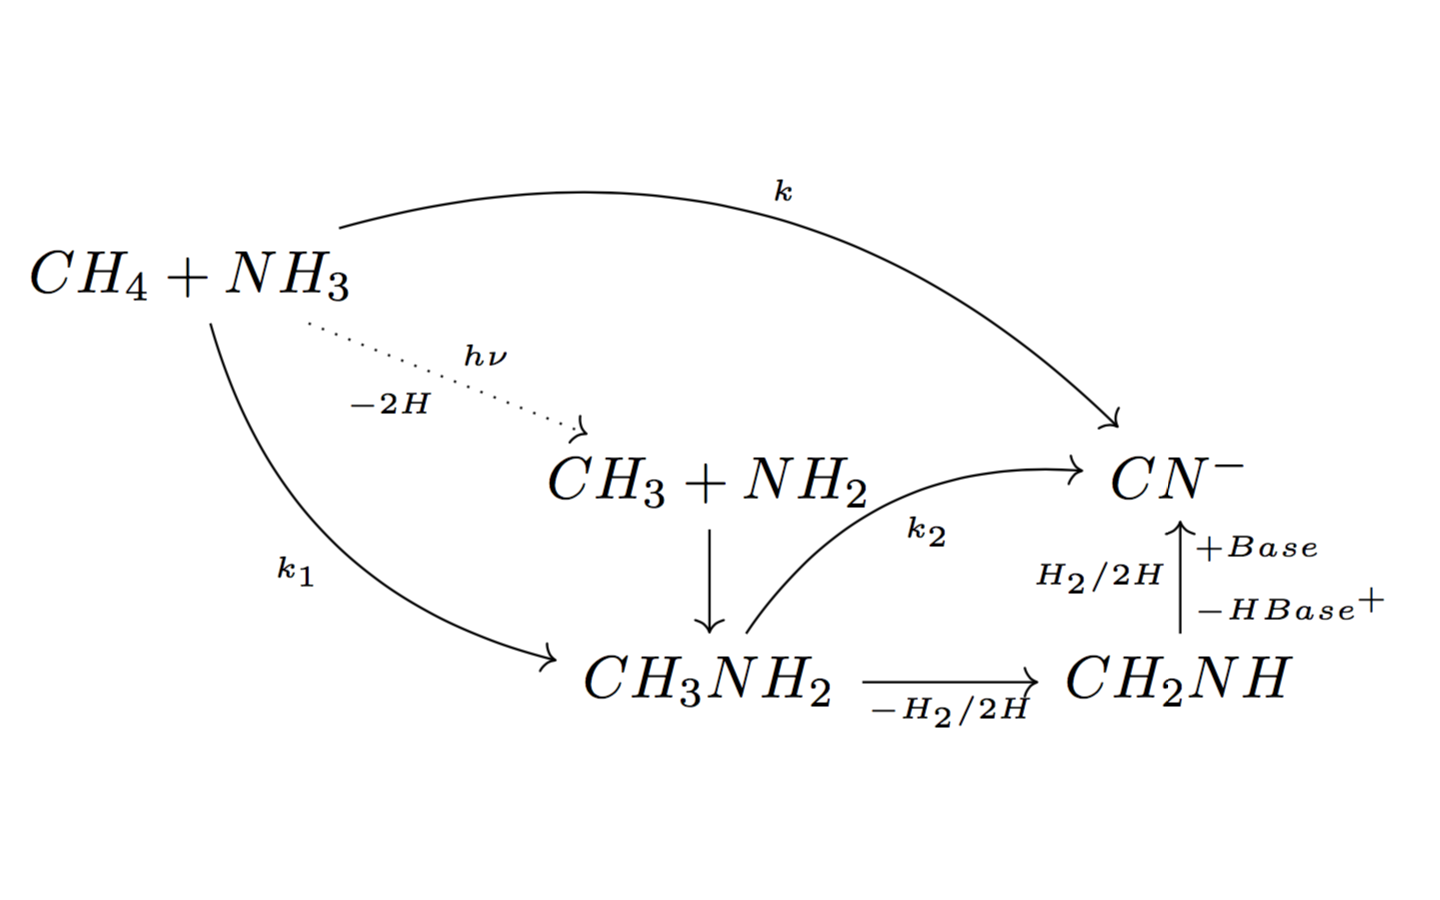
\includegraphics[width=\textwidth]{figures/chapter3/CNmechanism}
\caption{The formation mechanism of CN$^-$ proposed by Kim and Kaiser(2011)\cite{kim} .}
\label{fig:CNmechanism}
\end{figure}

The formation mechanism of CN$^-$ at low temperature was first suggested by Kim and Kaiser (2011) \cite{kim} to be two step reaction mechanism with methylamine as intermediate. CH$_4$ and NH$_3$ irradiated by photon become CH$_3$ and NH$_2$ radicals (figure \ref{fig:CNmechanism}), followed by propagation and recombination of radicals becoming CH$_3$NH$_2$ and dehydrogenation and acid-base reaction to form CN$^-$. \\

Kim and Kaiser (2011) \cite{kim} used 1.5 keV electron as energy source to simulate the cosmic ray induced photochemistry.  Despite the extra heats generated in these exothermal reactions:
\begin{equation}
CH_2 + NH_3 \rightarrow CH_3NH_2, \Delta H = -3.7 eV
\label{eq:methylamine_1}
\end{equation}
\begin{equation}
CH_4 + NH \rightarrow CH_3NH_2, \Delta H = -3.14 eV
\label{eq:methylamine_2}
\end{equation}
\begin{equation}
CH_3 + NH_2 \rightarrow CH_3NH_2, \Delta H = -3.64 eV
\label{eq:methylamine_3}
\end{equation}
Kundu et al. (2017) fails to observe methylamine as intermediate during warmup phase after using 1$-$90 eV electrons to initiate CH$_4$ and NH$_3$ ice mixtures\cite{kundu2017electron}. The non-detection is probably due to their thin ice thicknesses (just a few monolayers). This formation mechanism also applies in our photon irradiation experiments because we can also detect the methylamine during our warm-up phase. The ion fragment with m/z=31 is assigned as CH$_3$NH$_2$$^+$ and detectable in all ratios of our CH$_4$ + NH$_3$ experiments (figure \ref{Mass31}).\\

\begin{figure}
\centering
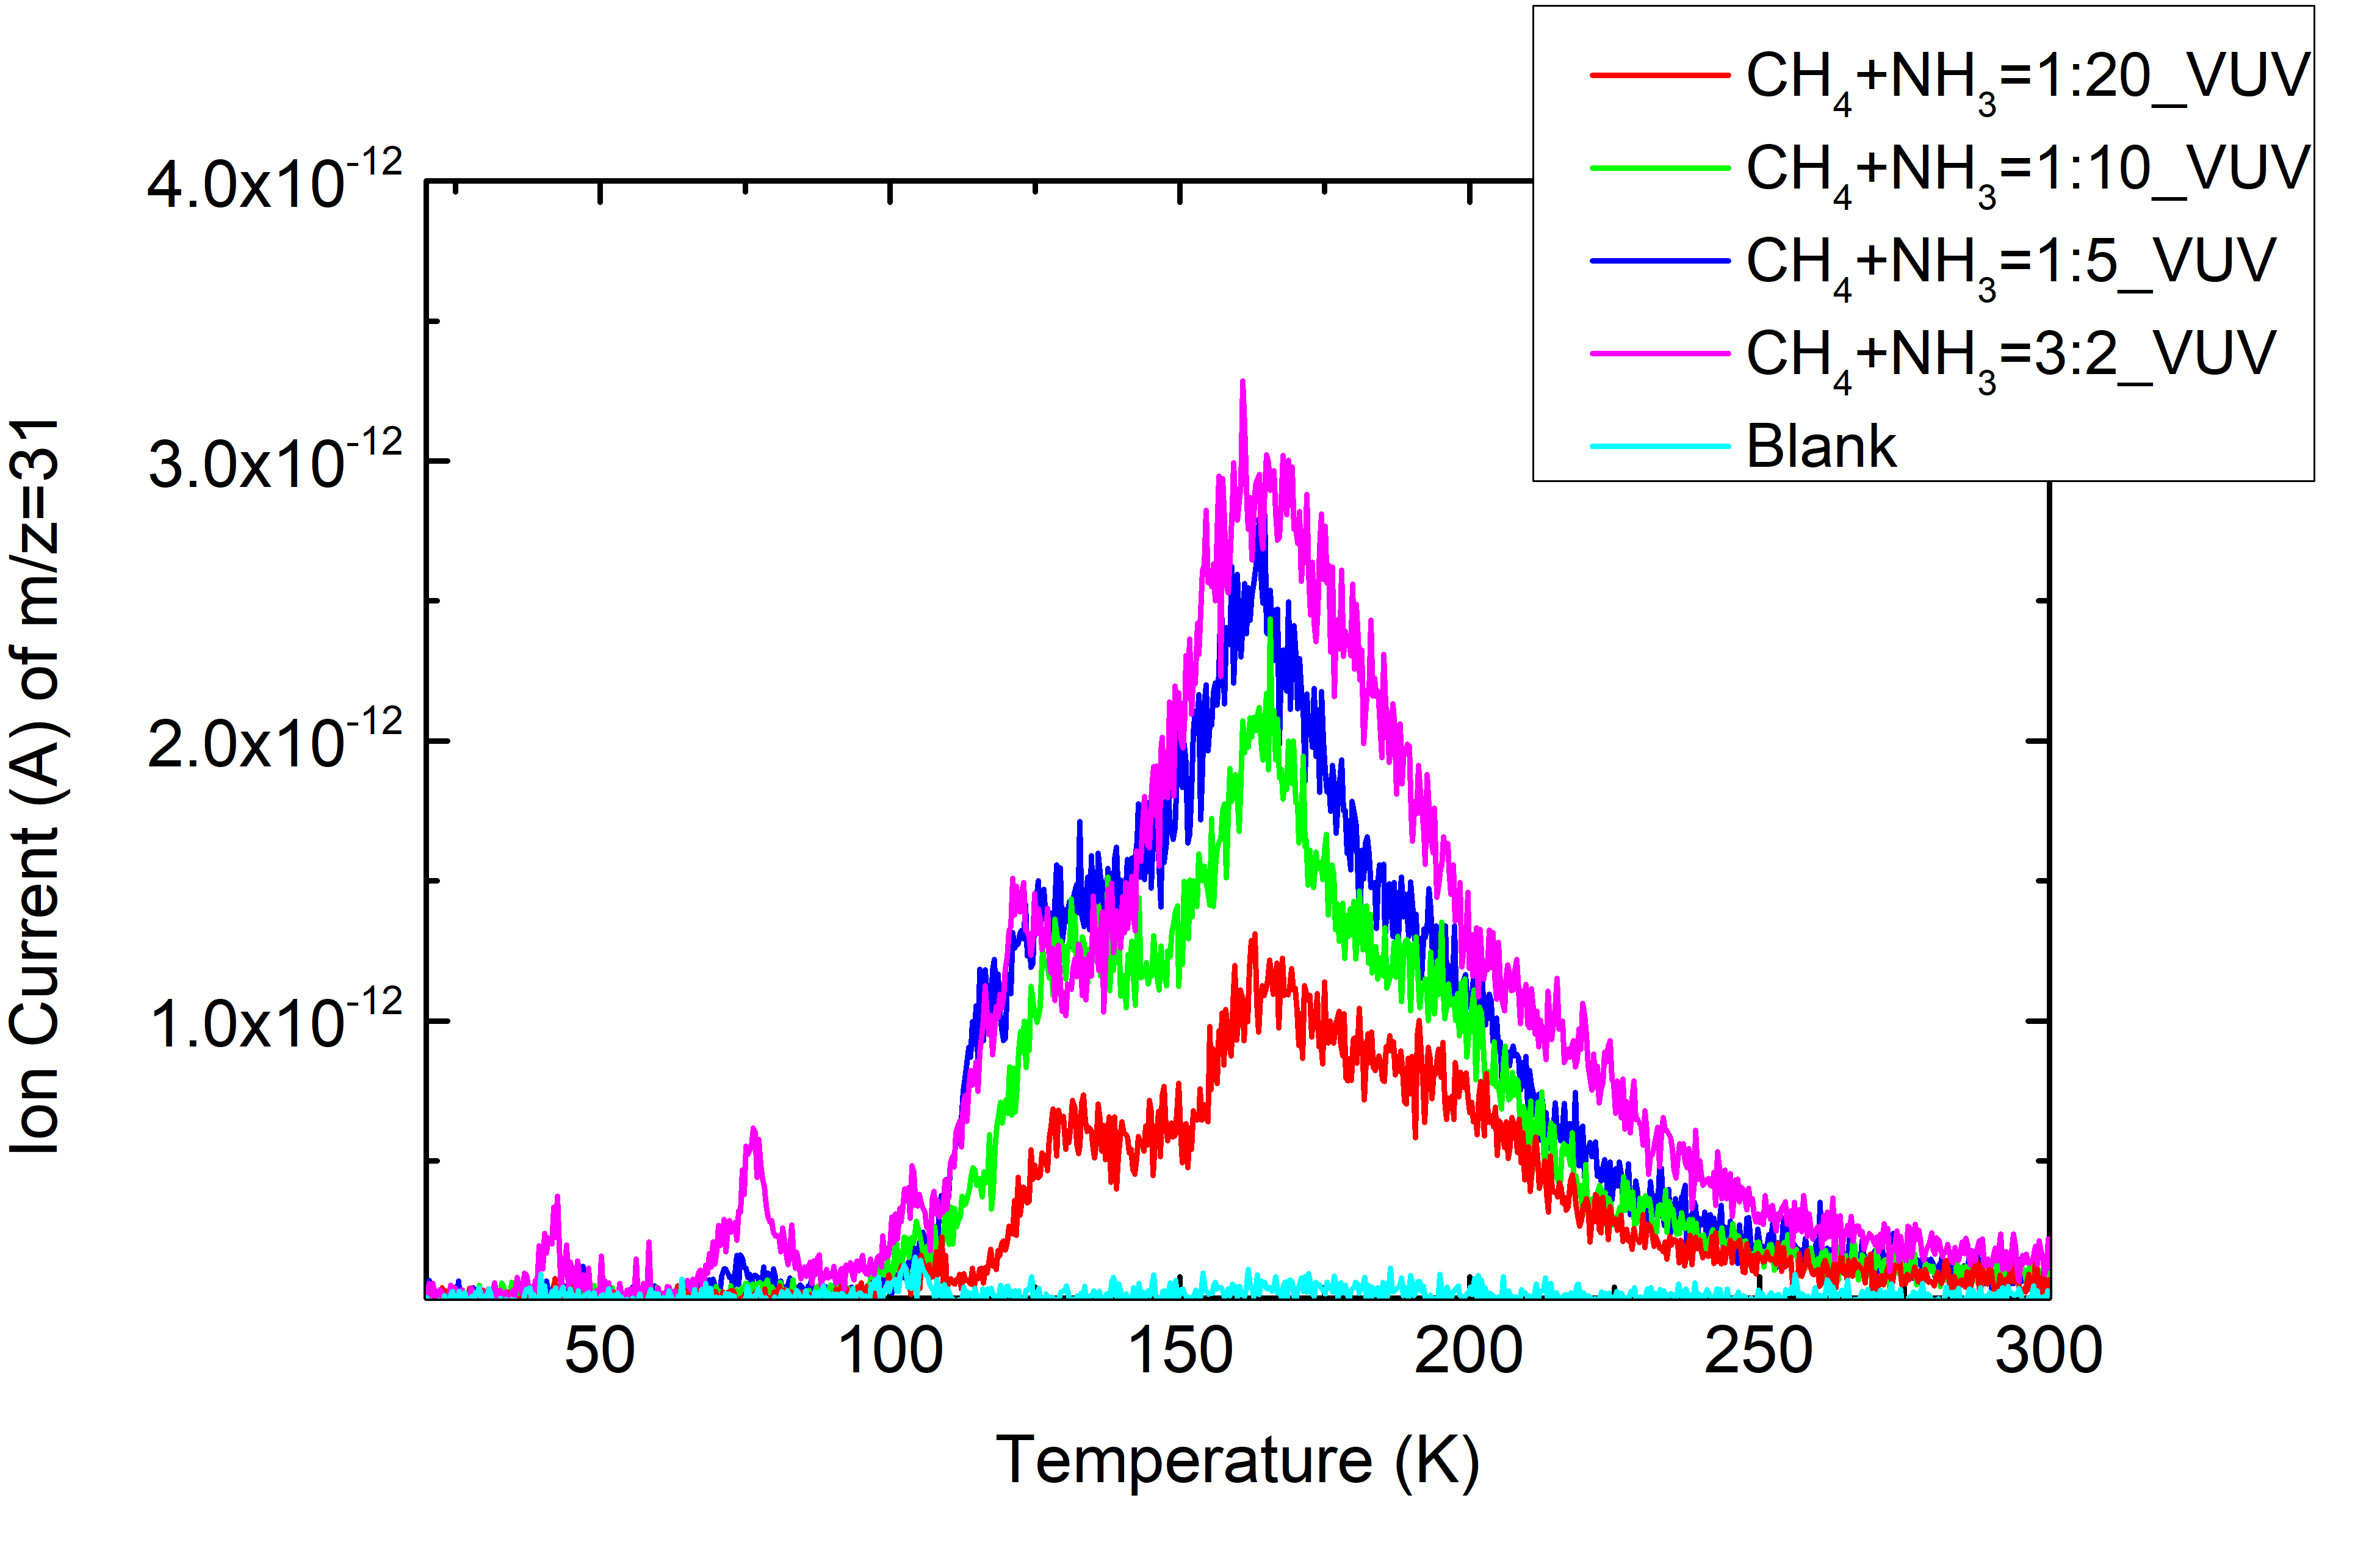
\includegraphics[width=\textwidth]{figures/chapter3/mass31.png}
\caption{The m/z=31 detected by QMS during warm-up with heating rate 1 K/min in different relative proportions of ice mixtures.}
\label{Mass31}
\end{figure}

By the deviations perform in section \ref{sec:Reaction_Rate_Laws}, we have a rate equation for consecutive reactions \ref{eq:rate7}. This rate equation applies in our experiments with one of the reactants in excess. Since CH$_4$ is more abundant than NH$_3$ (CH$_4$:NH$_3$=3:2); or NH$_3$ is in excess (CH$_4$:NH$_3$ = 1:5, 1:10 and 1:20) we may apply the pseudo first order assumption. Throughout the formation mechanism, one of the reactant (niether C or N) is a limiting reatant, therefore, we may apply the rate equation \ref{eq:rate7} to fit the formation of CN$^-$ (figure \ref{fig:CNrate}).\\

The fitting results are averaged by more than two experiments and are shown in table \ref{tab:CNrate}. We find that one of the rate constant is always larger than the other in all of the ratios. The results of Kim and Kaiser is also listed into the table, they could observe a two-step reaction mechanism in production of CN$^-$ in CH$_4$:NH$_3$ =3:1 experiments with electron current 0.1 $\mu$A. However, when they increase the electron flux to 1 $\mu$A for irradiating C$_n$H$_{2n+2}$ (n=1-6) and NH$_3$ ice mixtures, they also observe a one-step reaction mechanism.\\

\begin{figure}
\centering
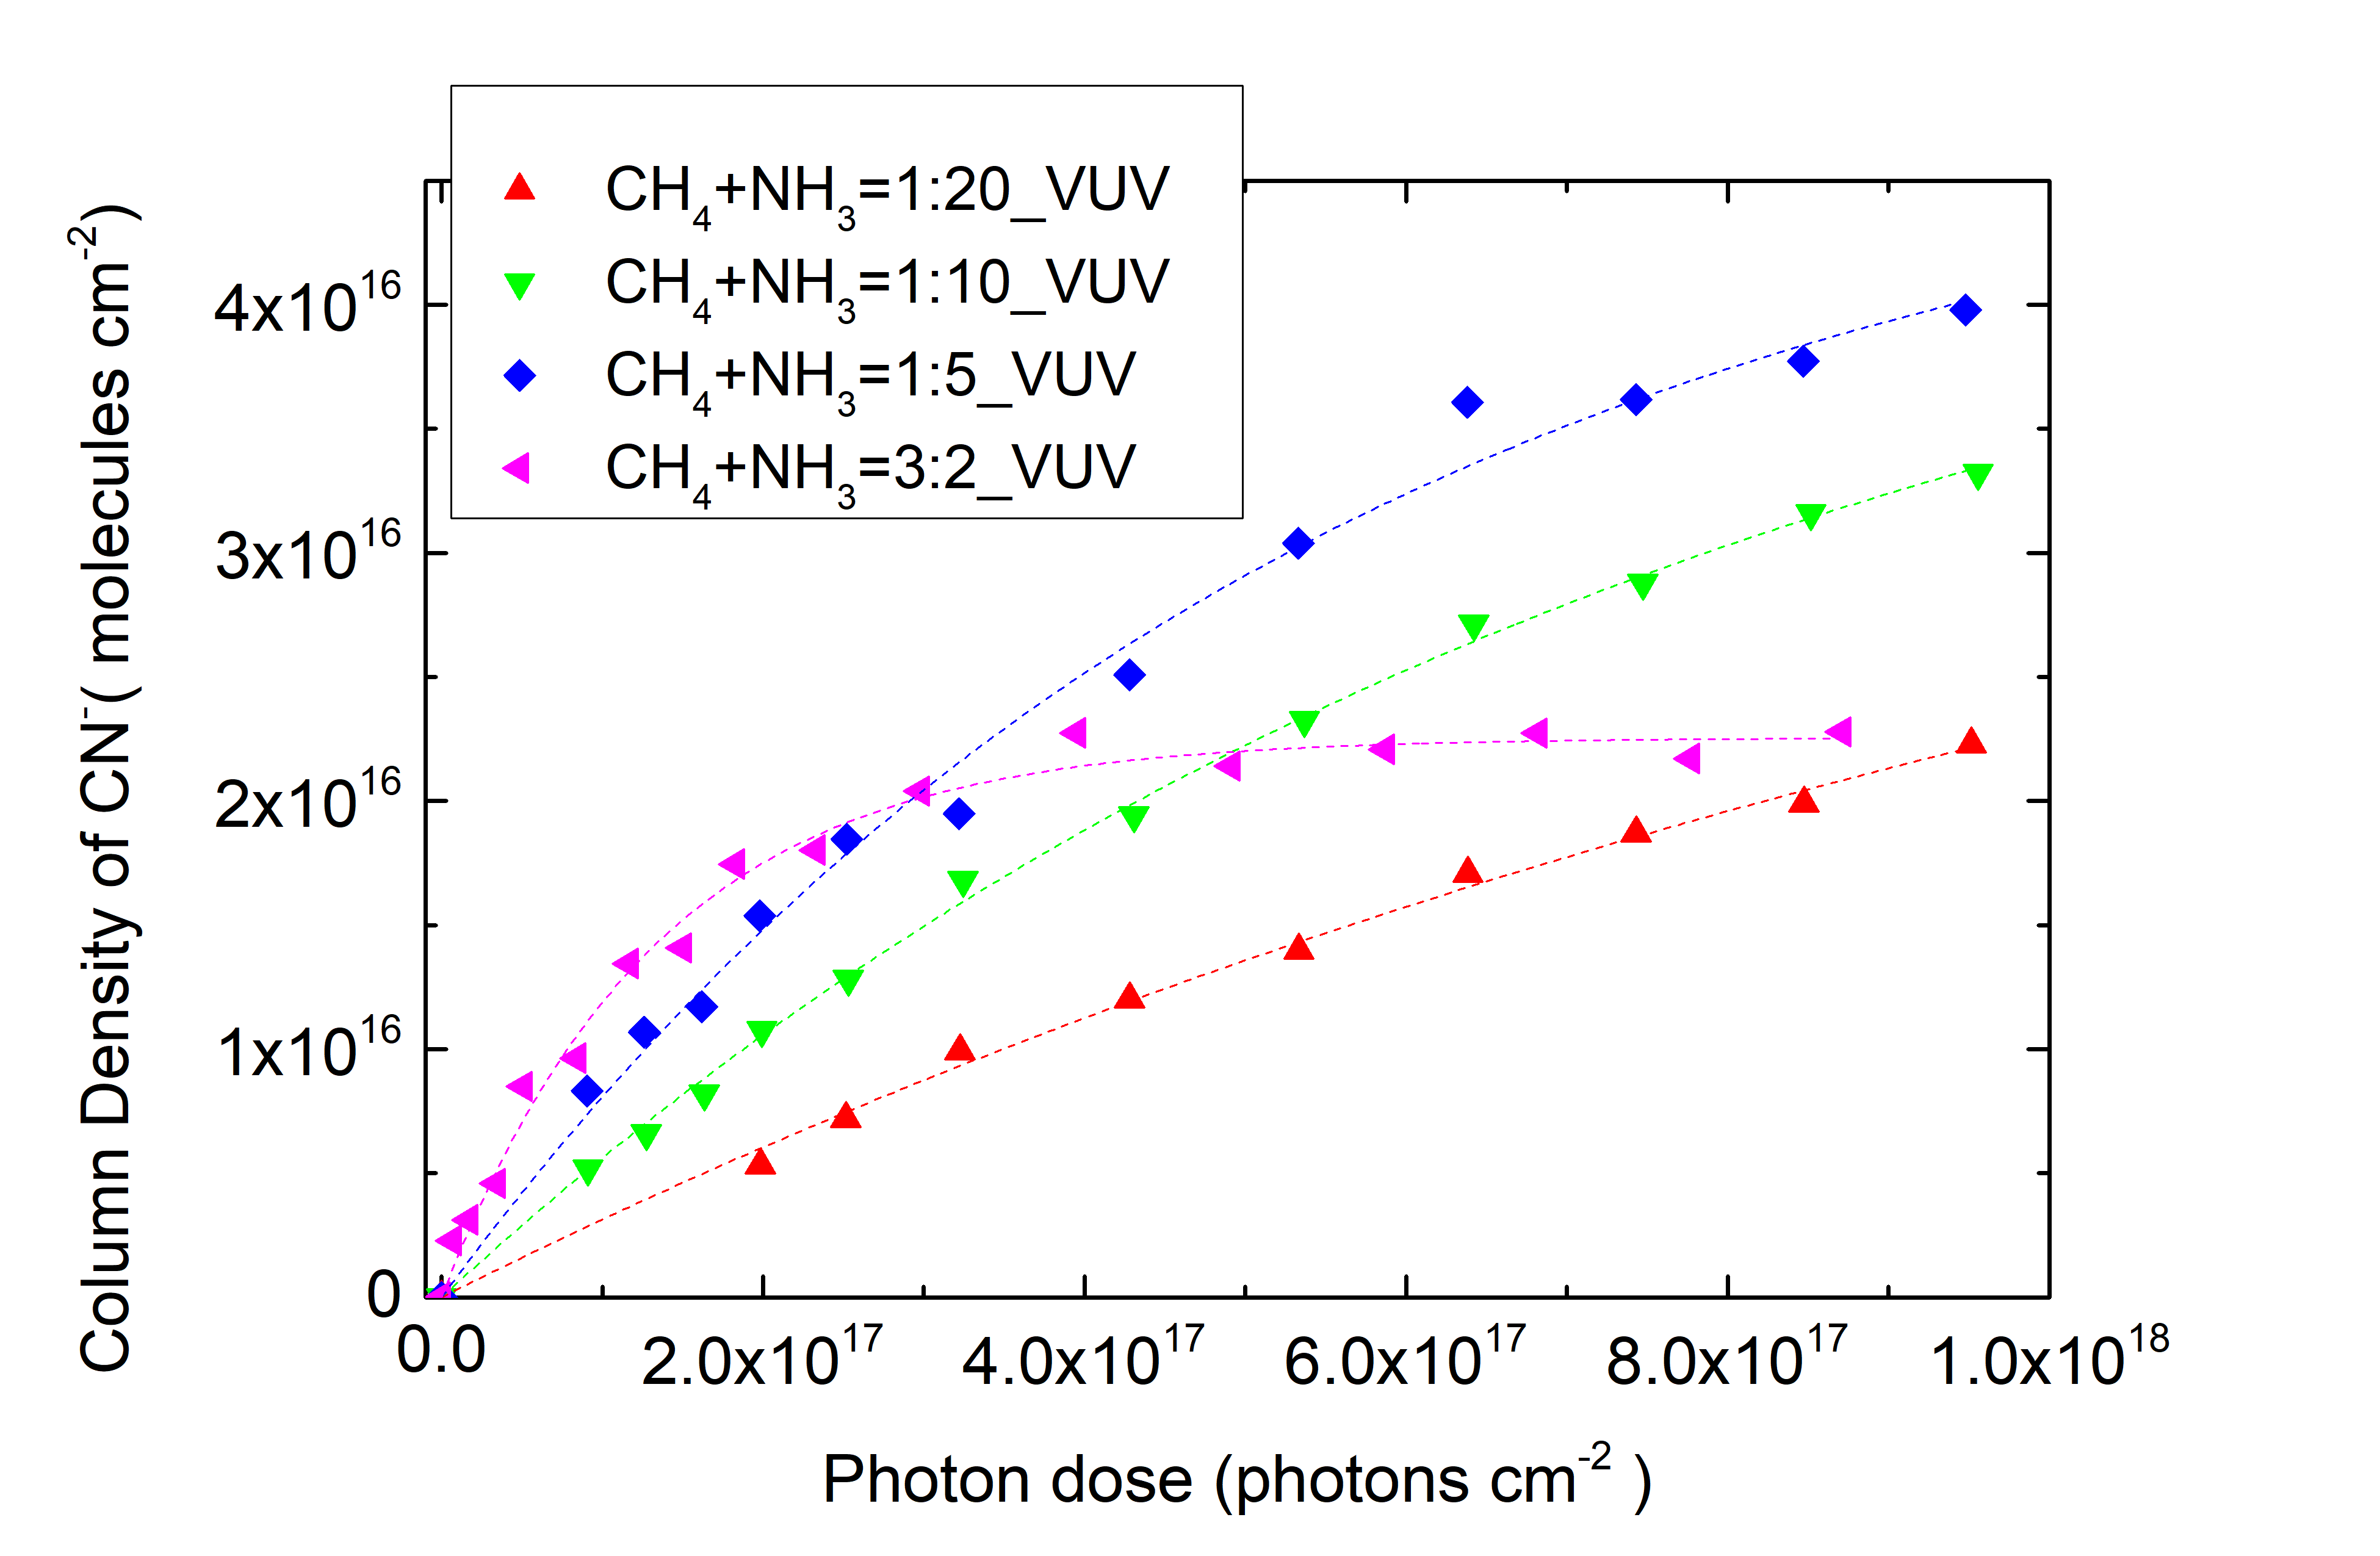
\includegraphics[width=\textwidth]{figures/chapter3/CN_rate_VUV.png}
\caption{The column density of CN$^-$ accumulated when different relative proportions of CH$_4$ + NH$_3$ ice mixtures are irradiated by VUV photons provided by MDHL. The dotted lines are fits of column densities by equation \ref{eq:rate7}.}
\label{fig:CNrate}
\end{figure}

\begin{table}[htbp]
\caption{The fitting results of CN$^-$ by equation \ref{eq:rate7}}
\label{tab:CNrate}
\begin{tabular}{cccc}
\hline
\hline
\multicolumn{4}{c}{VUV experiments with CH$_4$:NH$_3$ ice mixtures}\\
Ratio & A (x10$^{16}$ molecules cm$^{-2}$) & k$_1$ (x10$^{-18}$ photon$^{-1}$) & k$_2$ (photon$^{-1}$)\\
\hline
1:20 & 4.75 $\pm$ 0.40 & 0.70 $\pm$ 0.09 & >1 \\
1:10 & 4.51 $\pm$ 0.18 & 1.33 $\pm$ 0.13 & >1 \\
1:5 & 4.61 $\pm$ 0.18 & 1.93 $\pm$ 0.19 & >1 \\
3:2 & 2.24 $\pm$ 0.03 & 8.21 $\pm$ 0.70 & >1 \\
\hline
\hline
\multicolumn{4}{c}{Quotated from Kim and Kaiser\cite{kim}} \\
Ratio & A(x10$^{16}$ molecules cm$^{-2}$) & $k_1$ ($\times$ 10$^{-3}$ s$^{-1}$) &  $k_2$  ($\times$ 10$^{-3}$ s$^{-1}$)\\
\hline
\multicolumn{4}{c}{0.1 $\mu$A e$^-$ with CH$_4$:NH$_3$ ice mixtures}\\
3:1 & 1.3 $\pm$ 0.0 & 2.7 $\pm$ 0.3 & 8.9 $\pm$ 1.6 \\
\hline
\multicolumn{4}{c}{1 $\mu$A e$^-$ with C$_n$H$_{2n+2}$ (n=1-6)+NH$_3$ ice mixtures}\\
2:5 & 1.0 $\pm$ 0.0 & 8.7 $\pm$ 1.3 & >>1 \\
\hline
\end{tabular}\\
A represents the amount of CN$^-$ we may obtain when irradiated the ice for infinitely long.\
\end{table}

\section{The Concentration Effects in CN$^-$formation and the relation with C$_2$H$_6$ and C$_3$H$_8$}



\subsection{Cyanide ion and Ethane}

From table \ref{tab:CNrate}, we may observe that the rate k$_1$ is nearly proportional to the concentration of CH$_4$.  As CH$_4$ to NH$_3$ ratio increases in ammonia dominated ices, more CH$_4$ are involved in CH$_3$ radical formation, thus there are more CH$_3$ radicals to produce CH$_3$NH$_2$ intermediates(figure \ref{fig:NH3_dominated}).\\

\begin{figure}
\centering
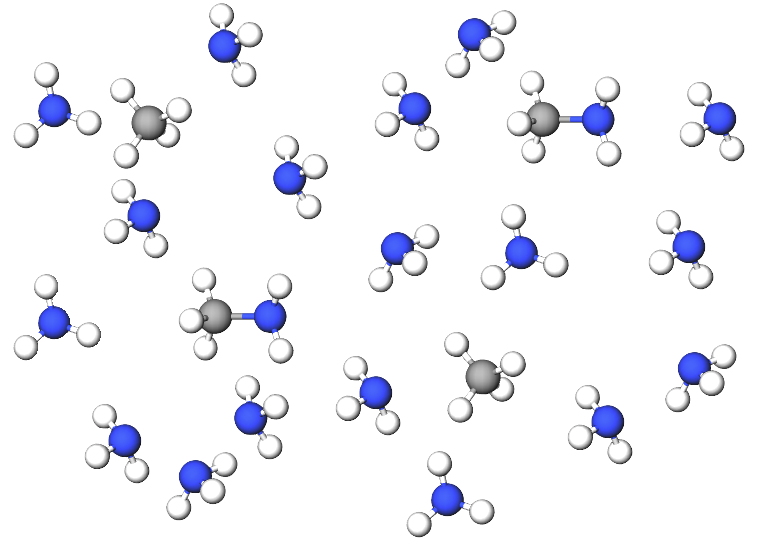
\includegraphics[width=0.5\textwidth]{figures/ammonia_dominating.png}
\caption{The NH$_3$ in excess situation where increasing CH$_4$ concentrations enhances the production of CN$^-$. The blue balls indicates N atoms, white balls indicates H atoms while grey ball is C atom.}
\label{fig:NH3_dominated}
\end{figure}


\begin{figure}
\centering
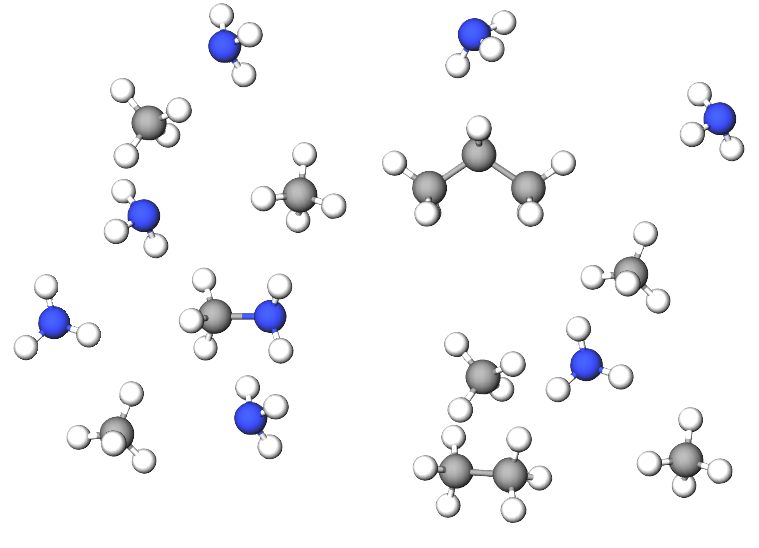
\includegraphics[width=0.5\textwidth]{figures/methane_dominating.png}
\caption{The CH$_4$ in excess situation where CH$_4$ reacts with neighbouring CH$_4$ molecules producing C$_2$H$_6$ and C$_3$H$_8$. The blue balls indicates N atoms, white balls indicates H atoms while grey balls are C atoms.}
\label{fig:CH4_dominated}
\end{figure}

In CH$_4$ to NH$_3$ =3:2 ice mixtures, the cyanide ion formed is about half of that of the other ratios. The decrease is mainly because NH$_2$ (forming CH$_3$NH$_2$) has a competing relationship with CH$_2$, CH$_3$ and C$_2$H$_4$ radicals (forming C$_2$H$_6$ and C$_3$H$_8$). This competition supresses the production of intermediate CH$_3$NH$_2$, thus the formation of CN$^-$ (figure \ref{fig:CH4_dominated}). Therefore, the yield of CN$^-$ is the least in CH$_4$ to NH$_3$ ice mixture with ratio 3:2 while the yield of C$_2$H$_6$ is the greatest in the mixture with the same ratio(table \ref{tab:CNrate}), (table \ref{tab:fittingC2H6}) Figure of CN$^-$ and C$_2$H$_6$ (figure \ref{fig:C2H6_CN_comparison}) shows the formation of CN$^-$ in ice mixtures with diluted CH$_4$ has more CN$^-$ formed than C$_2$H$_6$. It is because ice mixtures with with higher concentrations in CH$_4$ is more effective for one CH$_3$ radical to combine with another CH$_3$ radical. In contrast, CH$_3$ radicals formed in the ice mixtures with diluted CH$_4$ concentrations are aggregated by NH$_3$. Therefore, CN$^-$ is more efficient to form in ice mixtures with excess NH$_3$.\\


\begin{figure}
\centering
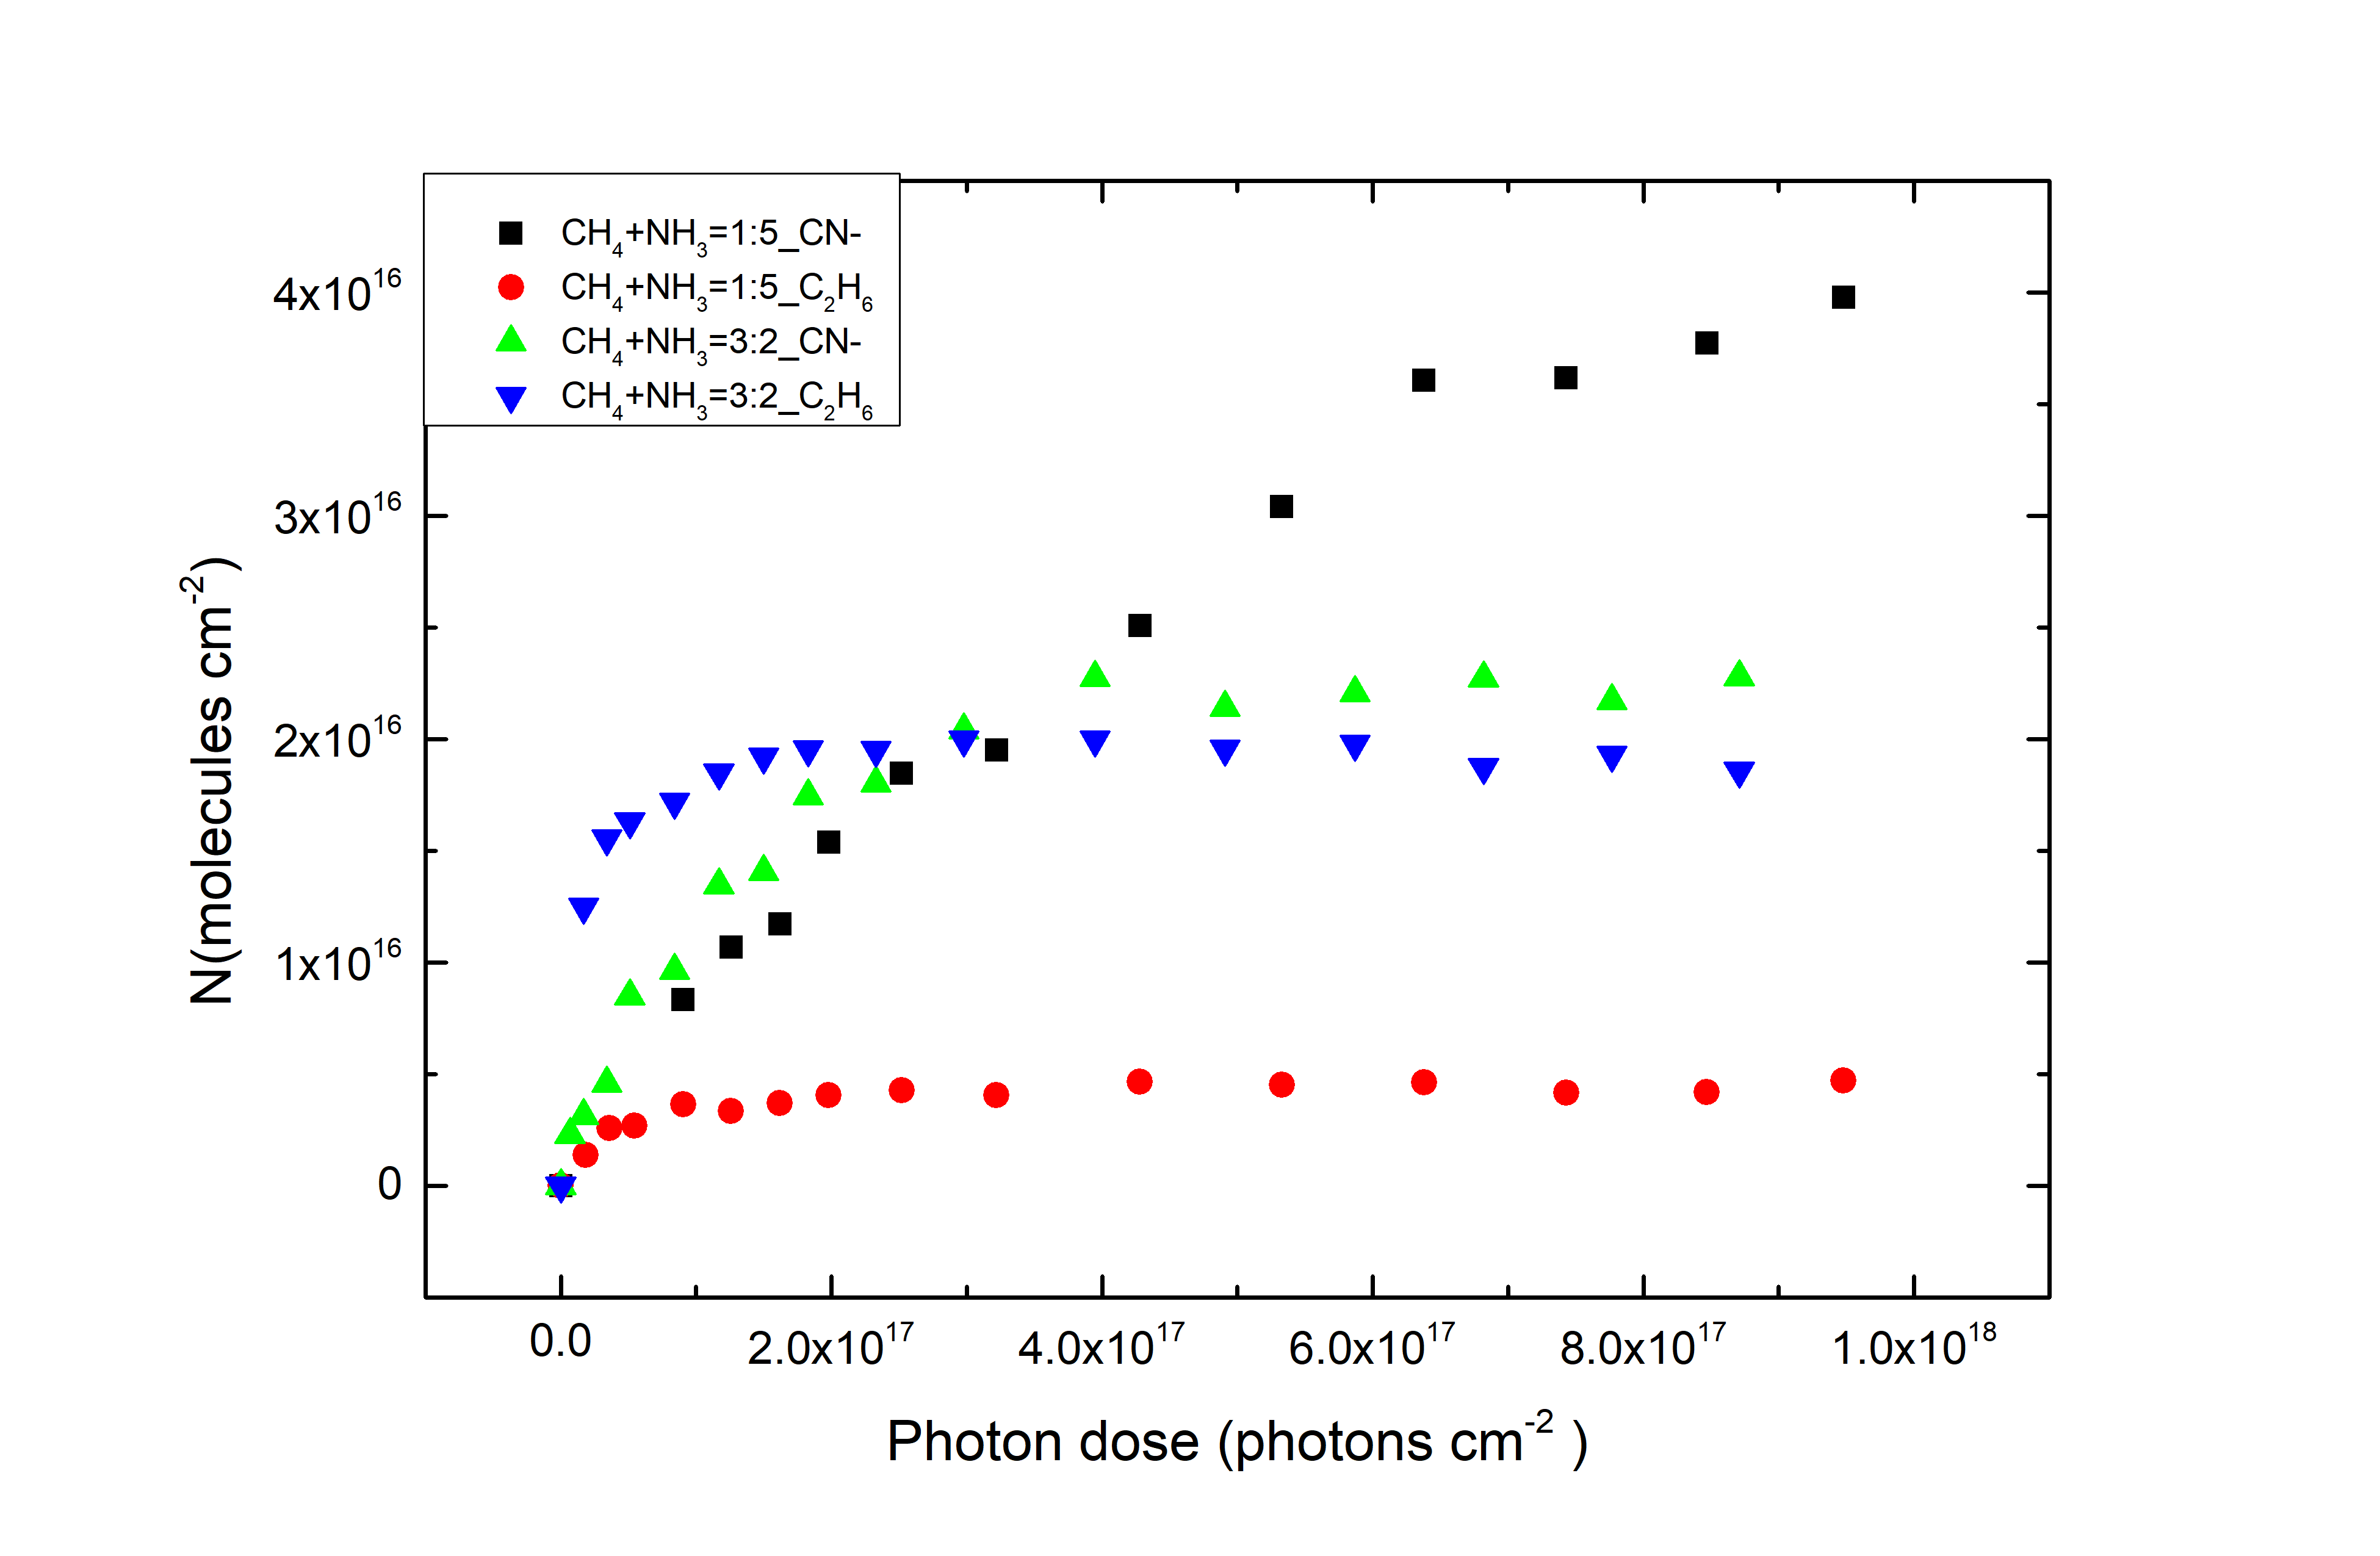
\includegraphics[width=\textwidth]{figures/chapter3/C2H6_CN_comparison.png}
\caption{The column density of CN$^-$ and C$_2$H$_6$ accumulated when different relative proportions of CH$_4$ + NH$_3$ ice mixtures are irradiated by VUV photons provided by MDHL.}
\label{fig:C2H6_CN_comparison}
\end{figure}


\section{Photon Energy Effect - EUV and VUV} %EUV & VUV

According to Blanksby and Ellison (2003) \cite{blanksby2003bond}, the dissociation energy for CH$_4$, becoming CH$_3$, CH$_2$, CH and C are 4.55, 4.79, 4.39 and 3.51 eV respectively at 298 K. Whereas dissociation energy for NH$_3$, becoming NH$_2$ is 4.67 eV at 298 K.\\

Considering our MDHL with average energy of 9.27 eV, all of the above fragments may exist either in the form of radicals or combine with other radicals to form heavier molecules in our ice mixtures. Although increasing the photon energy does not create new fragmentation pathway, the choice of fragmentation pathways depends on photon energy.\\

Several gaseous state measurements also support this statement. First, Gans et al. (2011) \cite{gans2011photolysis} changed VUV photon wavelengths from 121.6 nm (10. 2eV) to 118.2 nm (10.4eV) to dissociate the CH$_4$ molecules and ionize the fragments with the corresponding photon energy. Changing the output of the pulsed laser from 121.6 to 118.1 nm significantly changed the ratio of CH$_3^+$ and CH$_2^+$, produced from fragmentation, from 1: 1 to 1:2. This slight change of photon energy, from 10.2 eV to 10.4 eV has a significant change in the ratio between different pathways.\\

Second, an EUV fragmentation experiment done by Tsai et al. \cite{tsai1980mass} used 30.4 nm to photo-dissociate CH$_4$ and tested it by time$-$of$-$flight mass spectrometer yields CH$_3^+$: CH$_2^+$: CH$^+$: C$^+$ = 1 :0.32: 0.118: 0.0237 (Tsai 1980). Consider the ratios of CH$_3$ to CH$_2$ radicals, it is around 3 to 1, which is in contrast to the experiment results of Gans et al. (2011)\cite{gans2011photolysis}. Although both of them are gaseous state experimental results, it is uncertain whether increasing photon energy can produce more CH$_2$ radicals in ice mixtues.\\

Thirdly, a group varies ratios of CH$_4$ + NH$_3$ mixtures and irradiate with far UV irradiation at 134 nm \cite{bossard1980far}. However, this group only used gas chromatography to analyse the final products and their reaction is carried in gas phase in room temperature. We aware that the VUV absorption spectra of CH$_4$ in solid phases is different from gaseous phases \cite{cruz2014vacuum}, so the exact photo dissociation fragmentation ratios by EUV nor VUV irradiations in astronomical environments are still unknown. It is worthwhile for us to perform the experiment by EUV irradiation to see if  EUV irradiation can generate any new products on the surface of Charon, or any difference in yield. Despite the photon energy of our MDHL is enough to dissociate both the CH$_4$ and NH$_3$ molecules, we further increase photon energy to He II 30.4 nm to examine the differences in photo-products. \\

\begin{figure}
\centering
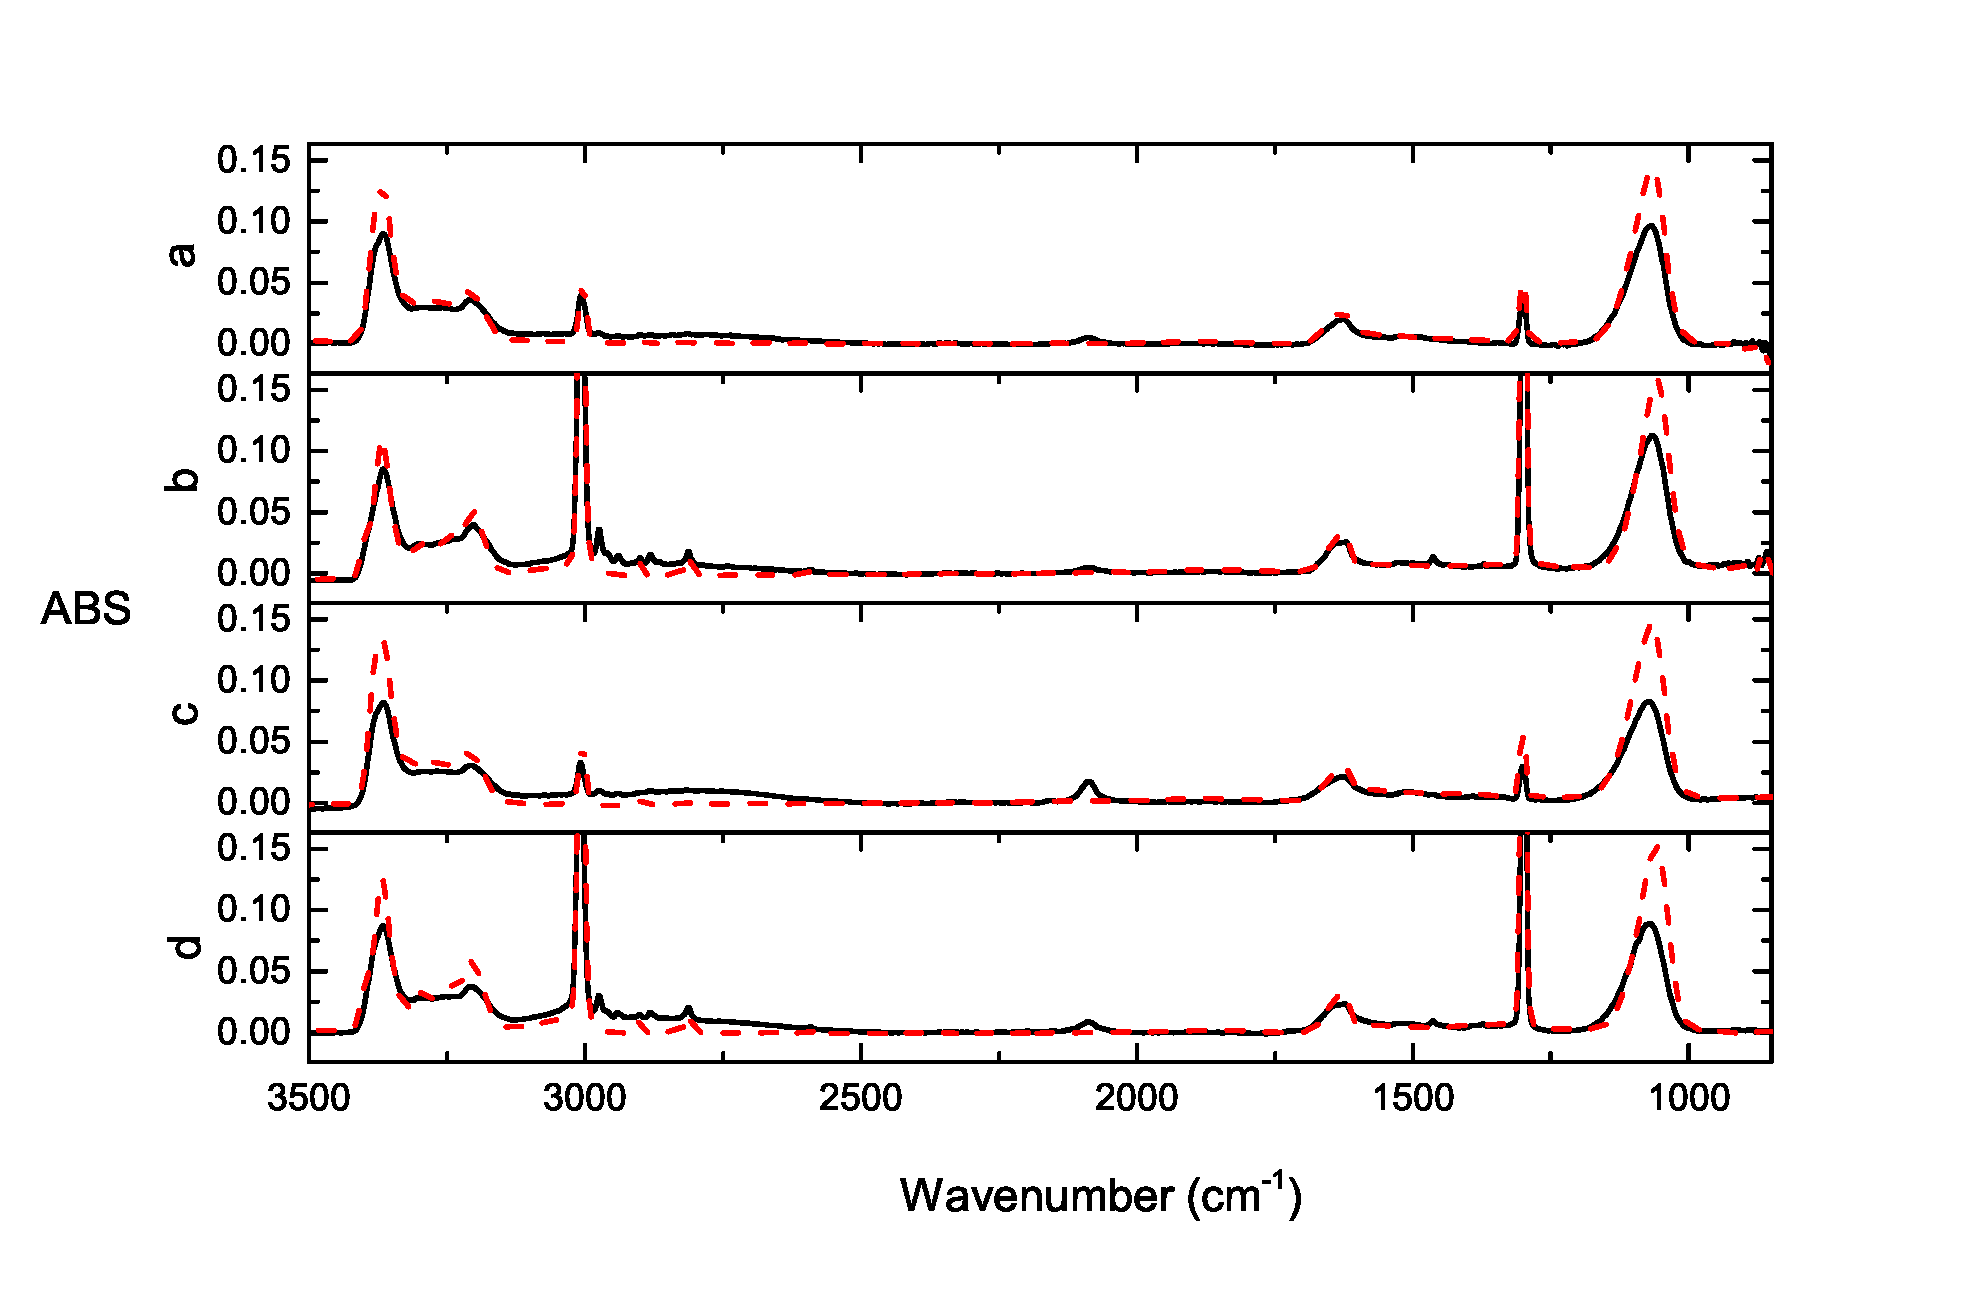
\includegraphics[width=\textwidth]{figures/chapter3/NSRRC_MDHL_IR.eps}
\caption{The the infrared spectrum of CH$_4$ + NH$_3$ ice mixtures before irradiation (black) and VUV and EUV (coloured) irradiated ice mixtures provided by MDHL. (a) and (b) are EUV irradiated CH$_4$:NH$_3$ = 1:5 and 3:2 ice mixtures respectively, and (c) and (d) are VUV irradiated CH$_4$:NH$_3$ = 1:5 and 3:2 ice mixtures respectively.}
\label{fig:NSRRC_MDHL_IR}
\end{figure}

Table \ref{tab:WavenumberNSRRC} shows the identified peaks of CH$_4$ + NH$_3$ ice mixtures irradiated by VUV and EUV (30.4 nm) irradiated in IR spectra (figure \ref{fig:NSRRC_MDHL_IR}).

\begin{table}[htbp]
\caption{The peak positions of identified substances after VUV and EUV irradiations in different relative proportions of ice mixtures.}
\label{tab:WavenumberNSRRC}
\begin{tabular}{ccccccc}
\hline
\hline
\multicolumn{2}{c}{Literture assignments} & \multicolumn{2}{c}{CH$_4$:NH$_3$ ratio (MDHL)} & \multicolumn{2}{c}{CH$_4$:NH$_3$ ratio (30.4 nm)} \\
\hline
Wavenumber & Identified IR modes  & 1:5 & 3:2 & 1:5 & 3:2 & Ref. \\
(cm$^{-1}$) &   & (cm$^{-1}$) & (cm$^{-1}$) & (cm$^{-1}$) & (cm$^{-1}$) &\\
\hline
3375 & $\nu_3$ (NH$_3$) & 3366 & 3367 & 3368 & 3368 & 1 \\
3210 & $\nu_1$ (NH$_3$) & 3207 & 3205 & 3209 & 3205 &1 \\
2972 & $\nu_{10}$ (C$_2$H$_6$) & 2975 & 2975 & 2977 & 2976 & 3 \\
2960 & C$_3$H$_8$ & - & 2960 & - & 2960 & 7 \\
2941 & $\nu_8+\nu_11$ (C$_2$H$_6$) & 2940 & 2940 & - & 2942 & 3 \\
2904 & $\nu_1$ (CH$_4$) & 2901 & 2901 & 2901 & 2901 & 5 \\
2879 & $\nu_5$ (C$_2$H$_6$) & 2882 & 2882 & - & 2884&  3 \\
2814 & $\nu_2+\nu_4$ (CH$_4$) & - & 2815 & - & 2813 & 5 \\
2083 & $\nu$ (CN$^-$) & 2088  & 2088 & 2090 & 2089 & 2 \\
1625 & $\nu_4$ (NH$_3$) & 1625 & 1631 & 1627 & 1631 & 1 \\
1514 & $\delta$ (NH$_2$) & 1509 & 1511 & 1509 & 1511 & 6 \\
1465-1440 & deform CH$_2$ scissor & 1461 & 1463 & - & 1465 & 3,4 \\
1390-1370 & CH$_3$ sym deform & 1394 & 1372 & - & 1372 & 4 \\
1298 & $\nu_4$ (CH$_4$) & 1301 & 1299 & 1303 & 1301 & 2 \\
1075 & $\nu_2$ (NH$_3$) & 1073 & 1072 & 1070 & 1068 & 1 \\
820 & $\nu_12$ (C$_2$H$_6$) & - & 820 & - & - & 3 \\
\hline
\end{tabular}\\
Reference: 1. Bossa et al. (2008) \cite{bossa2008carbamic} 2. Moore and Hudson (2003) \cite{moore2003infrared} 3. Kim et al. (2010) \cite{kim2010abiotic} 4. Socrates et al. (2001) \cite{socrates2001infrared} 5. Bennet and Kaiser (2007) \cite{bennett2007formation} 6. Zheng et al. (2008) \cite{zheng2008formation} 7. Hudson and Moore (2004) \cite{hudson2004reactions}
\end{table}


\begin{figure}
\centering
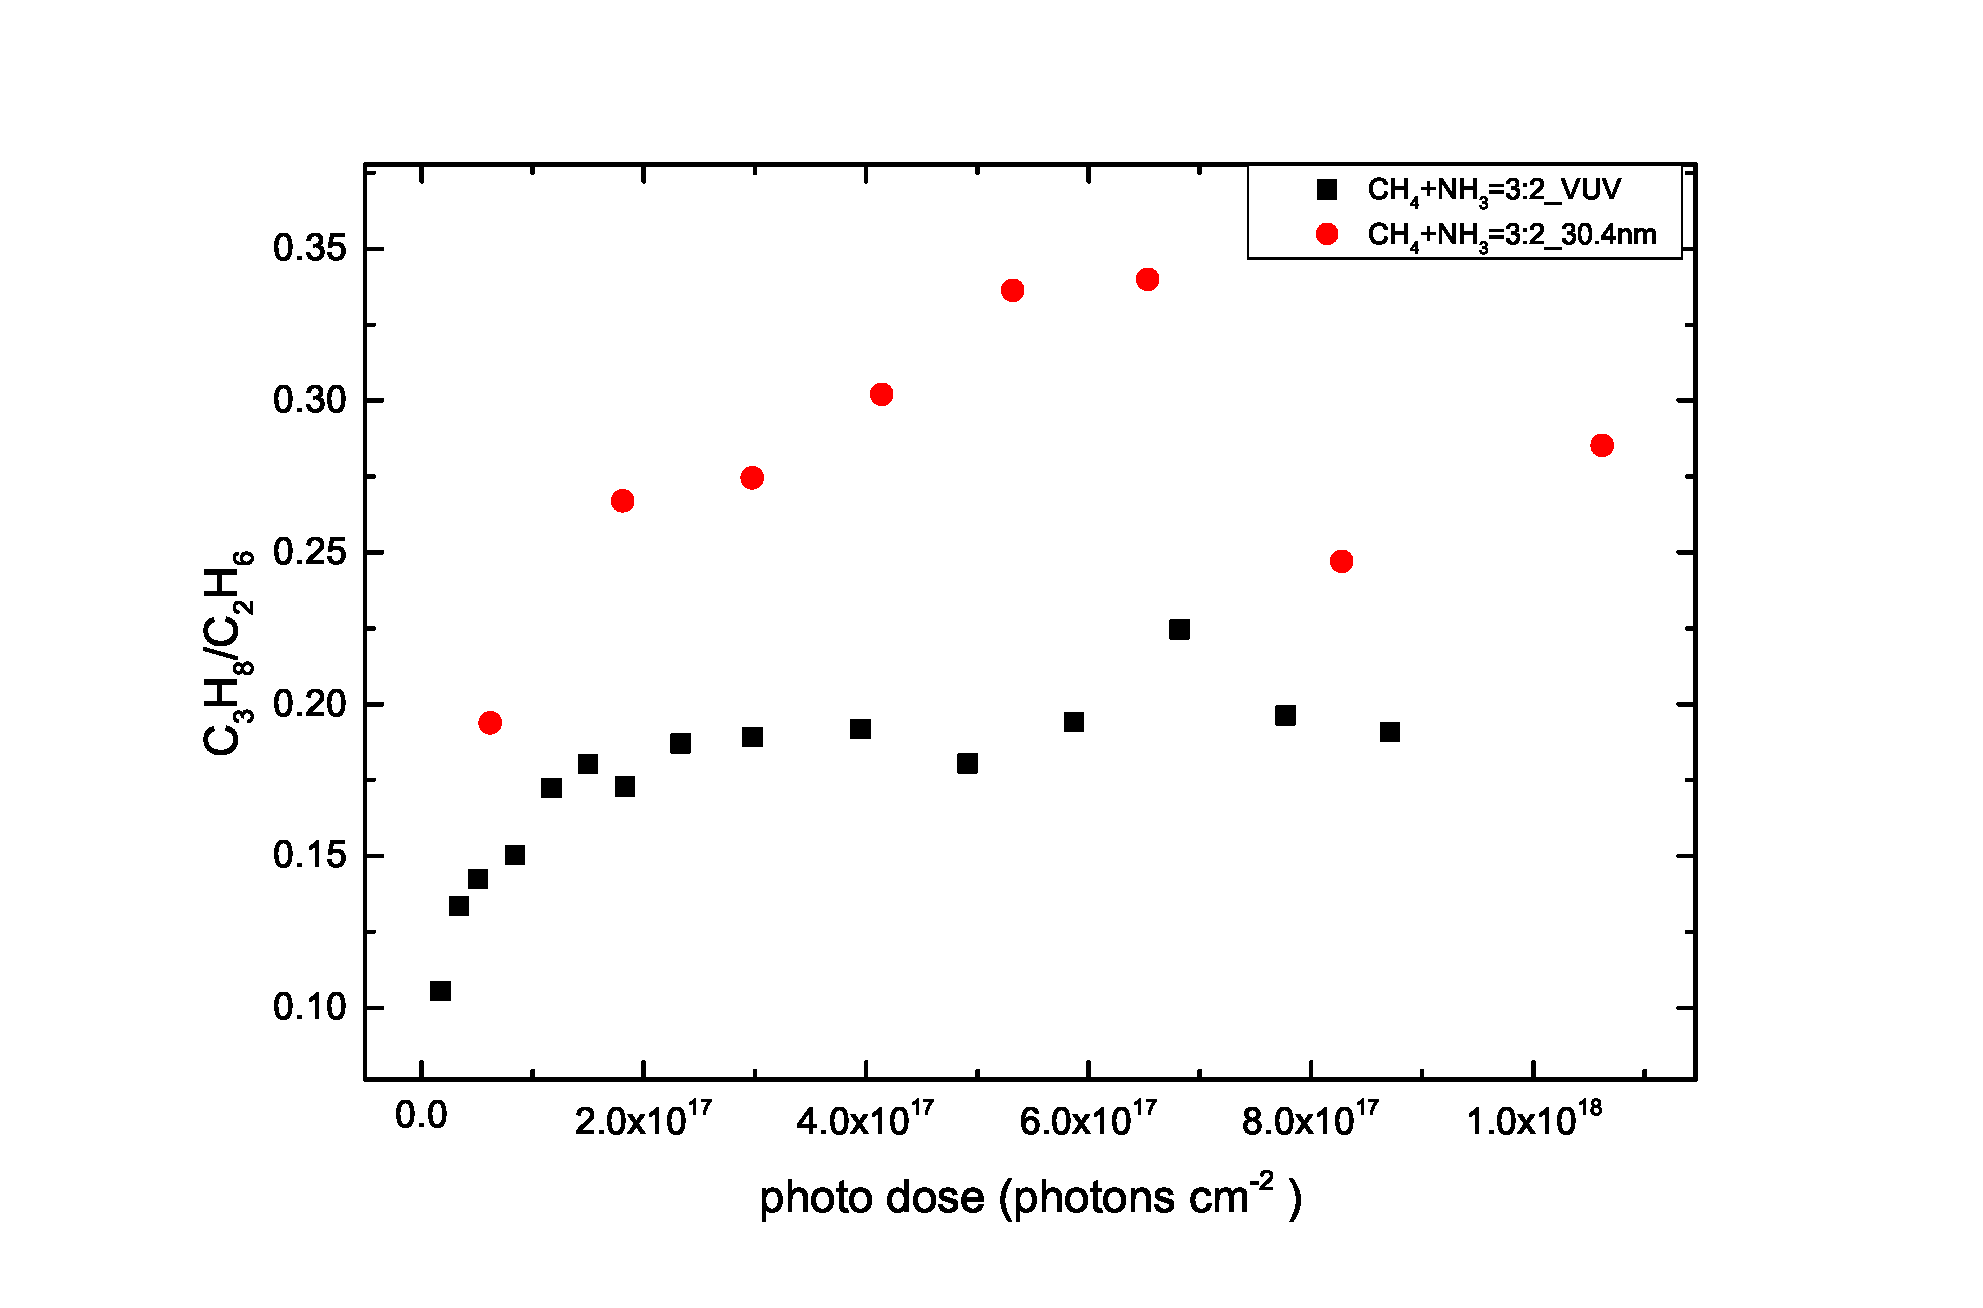
\includegraphics[width=\textwidth]{figures/chapter3/NSRRC_Lab_C3H8_C2H6.eps}
\caption{The column density of C$_3$H$_8$ divided by C$_2$H$_6$ accumulated when different relative proportions of CH$_4$ + NH$_3$ ice mixtures are irradiated by VUV and EUV photons}
\label{fig:NSRRC_Lab_C3H8_C2H6}
\end{figure}


From figure \ref{fig:NSRRC_Lab_C3H8_C2H6}, we may observe that more C$_3$H$_8$ is produced by 30.4nm (40.8 eV) photons than by VUV photons. Considering the formation mechanisms of C$_2$H$_6$ and C$_3$H$_8$, equation (\ref{eq:C2H6} and \ref{eq:C3H81}), when MDHL VUV irradiation is replaced by He II 30.4 nm monochromatic light, the ratio of C$_3$H$_8$ to C$_2$H$_6$ in CH$_4$ to NH$_3$ = 3:2 ice mixtures irradiated by VUV irradiation is lower under EUV irradiation than that  under EUV provided by NSRRC (figure \ref{fig:NSRRC_Lab_C3H8_C2H6}). There are many possible explanations, one of those maybe the internally excited C$_2$H$_6$ can break down to be C$_2$H$_4$, which implies the production of C$_3$H$_8$. Second, it may be caused by the increase in CH$_2$ radicals during fragmentation of CH$_4$, from the findings of Gans et al. (2011)\cite{gans2011photolysis}, the ratio of CH$_2$ radicals increases from 0.3 to 0.48 when photon energy increases from 121.6 nm to 118.2 nm in their pulsed laser experiments.\\


\begin{figure}
\centering
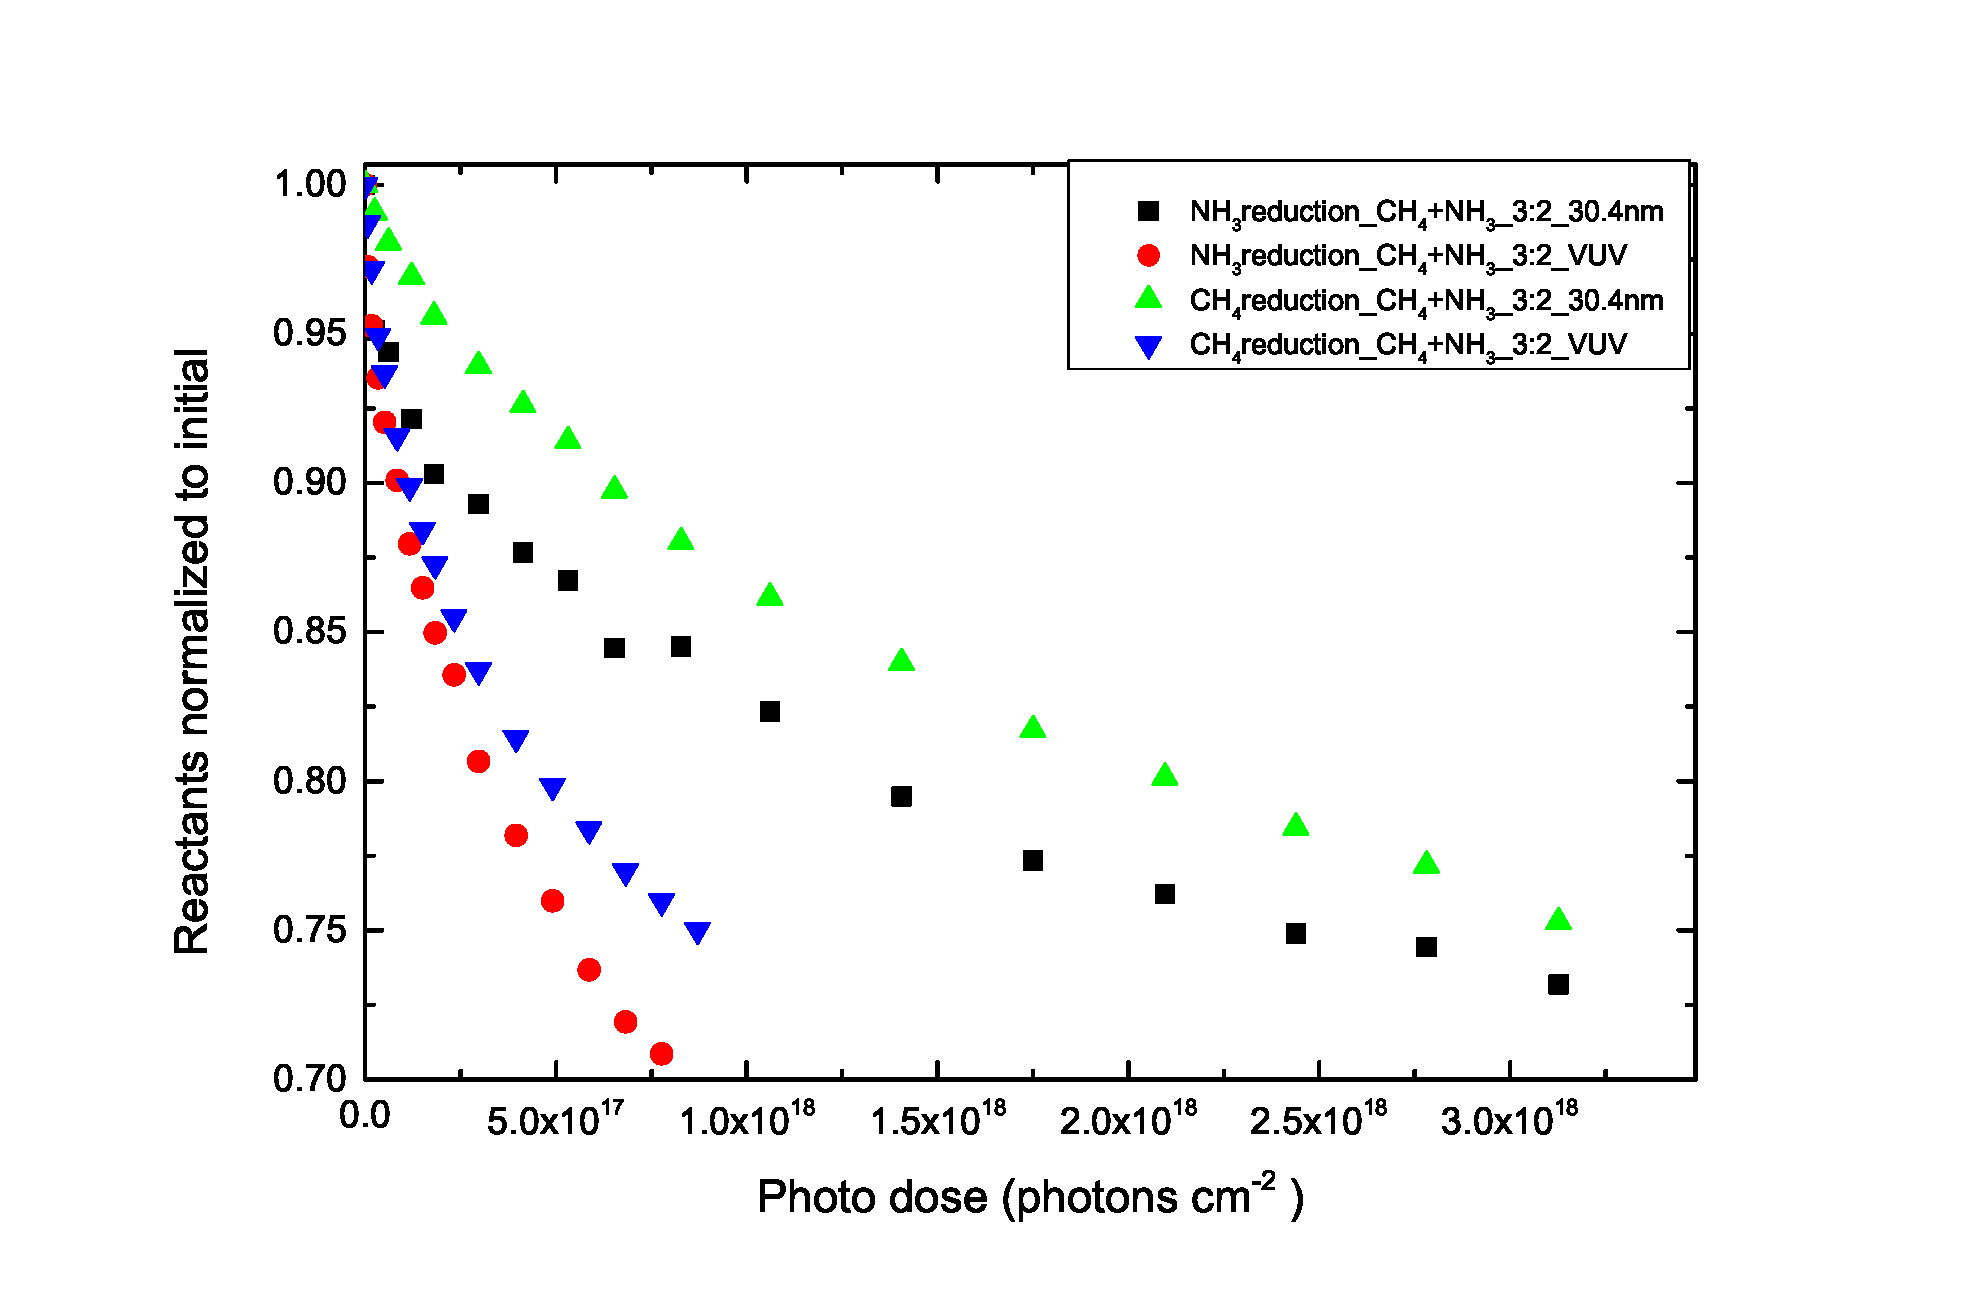
\includegraphics[width=\textwidth]{figures/chapter3/Reactants_normalized_to_initial.eps}
\caption{The normalized destruction of CH$_4$ and NH$_3$ in CH$_4$ + NH$_3$ ice mixtures irradiated by VUV and EUV photons}
\label{fig:normalized_reactants}
\end{figure}

Apart from C$_2$H$_6$ and C$_3$H$_8$, are there any difference in CN$^-$ production? Figure \ref{fig:CN_NSRRC} shows the accumulated column densities of CN$^-$ generated by irradiation of CH$_4$+NH$_3$ ice mixtures by MDHL and 30.4 nm monochromatic light. The fitting results are shown in Table 3.6. The rate constants forming CN$^-$ is 3.06 to 4.13 times larger in CH$_4$:NH$_3$ = 1:5 and 3:2 irradiated by MDHL than irradiated by 30.4 nm monochromatic light respectively. From figure \ref{fig:normalized_reactants}, the destruction cross-section of CH$_4$ and NH$_3$ are reduced by 6.06$\pm$0.07 and 3.19$\pm$0.12 times respectively. The formation rate constants of CN$^-$ is 3.06 to 4.13 times smaller than VUV irradiations (table \ref{tab:CNrate_NSRRC}. Therefore, we may conclude that the decrease in CN$^-$ formation rate by 30.4nm (40.8 eV) EUV irradiation is mainly due to the decreased NH$_3$ destruction cross-sections. In general, the energy of MDHL has already exceeded the energy required to form the CH$_3$ and NH$_2$ radicals, further increasing photon energy would not pose dramatical change to CH$_4$ and NH$_3$ ice mixtures.\\

\begin{figure}
\centering
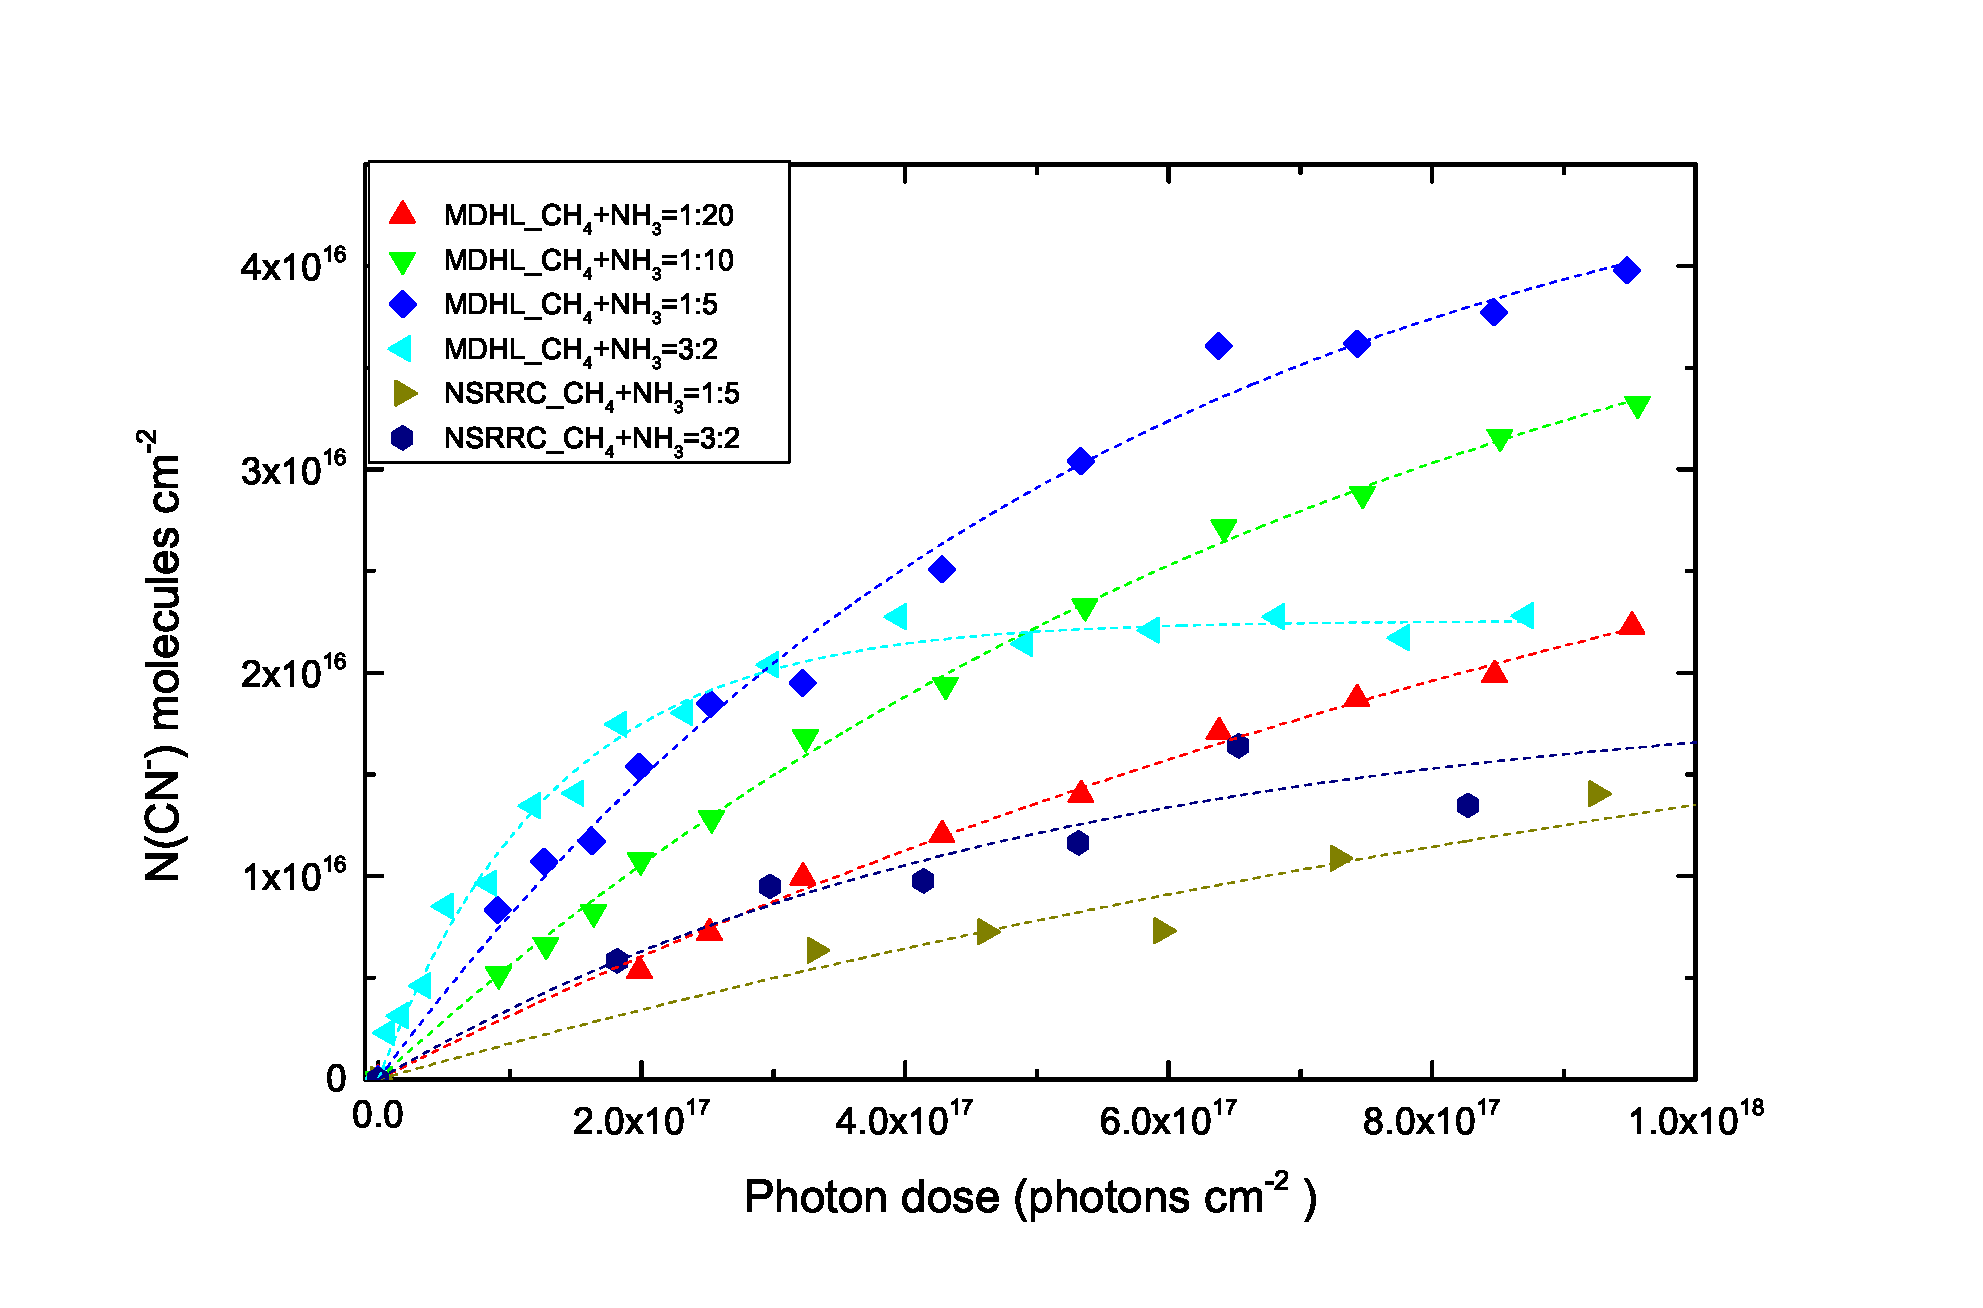
\includegraphics[width=\textwidth]{figures/chapter3/overall_CN_NSRRC.eps}
\caption{The column densities of CN$^-$ generated by irradiation of CH$_4$+NH$_3$ ice mixtures by MDHL and 30.4 nm monochromatic light.}
\label{fig:CN_NSRRC}
\end{figure}

\begin{table}[htbp]
\caption{The fitting results of CN$^-$ by equation \ref{eq:rate7}}
\label{tab:CNrate_NSRRC}
\begin{tabular}{ccccc}
\hline
\hline
Light source & Ratio of CH$_4$:NH$_3$ & A (x10$^{16}$ molecules cm$^{-2}$) & k$_1$ (x10$^{-18}$ photon$^{-1}$) & k$_2$ (photon$^{-1}$)\\
\hline
VUV & 1:5 & 4.61 $\pm$ 0.18 & 1.93 $\pm$ 0.19 & >1 \\
MDHL & 3:2 & 2.24 $\pm$ 0.03 & 8.21 $\pm$ 0.70 & >1 \\
\hline
EUV & 1:5 & 2.89 $\pm$ 1.29 & 0.63 $\pm$ 0.37 & >1 \\
 30.4nm & 3:2 & 2.24 $\pm$ 0.03 & 1.92 $\pm$ 1.99 & >1 \\
\hline
\end{tabular}
Fitting result of figure \ref{fig:CN_NSRRC} with pseudo first order equation [CN$^-$]=$A(1-e^{-kx})$. These fitting results of MDHL experiments are an average of at least 2 experiments with the same circumstances. In the expression, A represents the column density when x, the photon dose, becomes infinitely large and k is the rate constant.\
\end{table}


\section{Residues}

The residues we studied are the accumulated substances remained on the substrate after warmed up. Figure \ref{fig:residues} is a comparison of CH$_4$:NH$_3$ = 3:2 after VUV experiments, residues accumulate after EUV exposure of CH$_4$:NH$_3$ = 3:2 ice mixtures and the plasma experiment done by Imanaka et al. (2004)\cite{imanaka2004laboratory}. The peak positions and assignments are listed at table \ref{rab:residue}. The residues formed in irradiated ammonia dominating CH$_4$+NH$_3$ ice mixtures is not observed after accumulation of consecutive experiments. There are no differences between EUV accumulated residues and VUV accumulated residues in CH$_4$:NH$_3$ = 3:2 ice mixtues. The main functional groups (nitrogen position) of the residues are conjugated nitriles. Based on experiments of N$_2$+CH$_4$ (9:1) done at 2300 Pa. by Imanaka et al. (2004)\cite{imanaka2004laboratory}, the tholins formed at high pressure (2300 Pa) should be a polymer-like branched chain structure terminated with -CH$_3$ -NH$_2$ and -C$\equiv$N with few aromatic compounds.\\

\begin{table}[htbp]
\caption{The peak positions of residues and their assignments}
\label{tab:residue}
\begin{tabular}{cccc}
\hline
\hline
Imanaka et al. & implied functional group & VUV (MDHL) & EUV (30.4 nm)\\
(2004) $\nu$ (cm$^{-1})$ & & $\nu$ (cm$^{-1})$ & $\nu$ (cm$^{-1}$) \\
\hline
2954 - 2972 & -CH$_3$- asymmetric stretching & 2955 & 2962 \\
2929 - 2932 & -CH$_2$- assymmetric stretching & 2923 & 2929 \\
2869 - 2874 & -CH$_3$- symmetric stretching & 2871 & 2871 \\
2173 - 2189 & conjugated nitriles, & 2173 & 2174 \\
 & such as with -C=C(-NH$_2$)& & \\
 & C-N$\equiv$C stretching& & \\
1460 & C-CH$_3$ asymmetric bending & 1451 & 1451 \\
1375-1379 & C-CH$_3$ unbrella symmetric bending & 1372 & 1378 \\
\hline
\end{tabular}
\end{table}

We may get similar residues by using different initial reactants (replacing N$_2$ by NH$_3$). The similarities during formation of atomic nitrogens when breaking N$\equiv$N bonds in nitrogen molecules (N$_2$) and N-H bonds in ammonia give rise to this result. When photon energy is enough to break both NH bond and N$\equiv$N bond, similar experimental residues forms. Our results implies that the residues formed on Charon is similar to what we found on Titan, although their formation environments differs from gaseous phase with N$_2$ dominating to solid phase with NH$_3$.\\

\begin{figure}
\centering
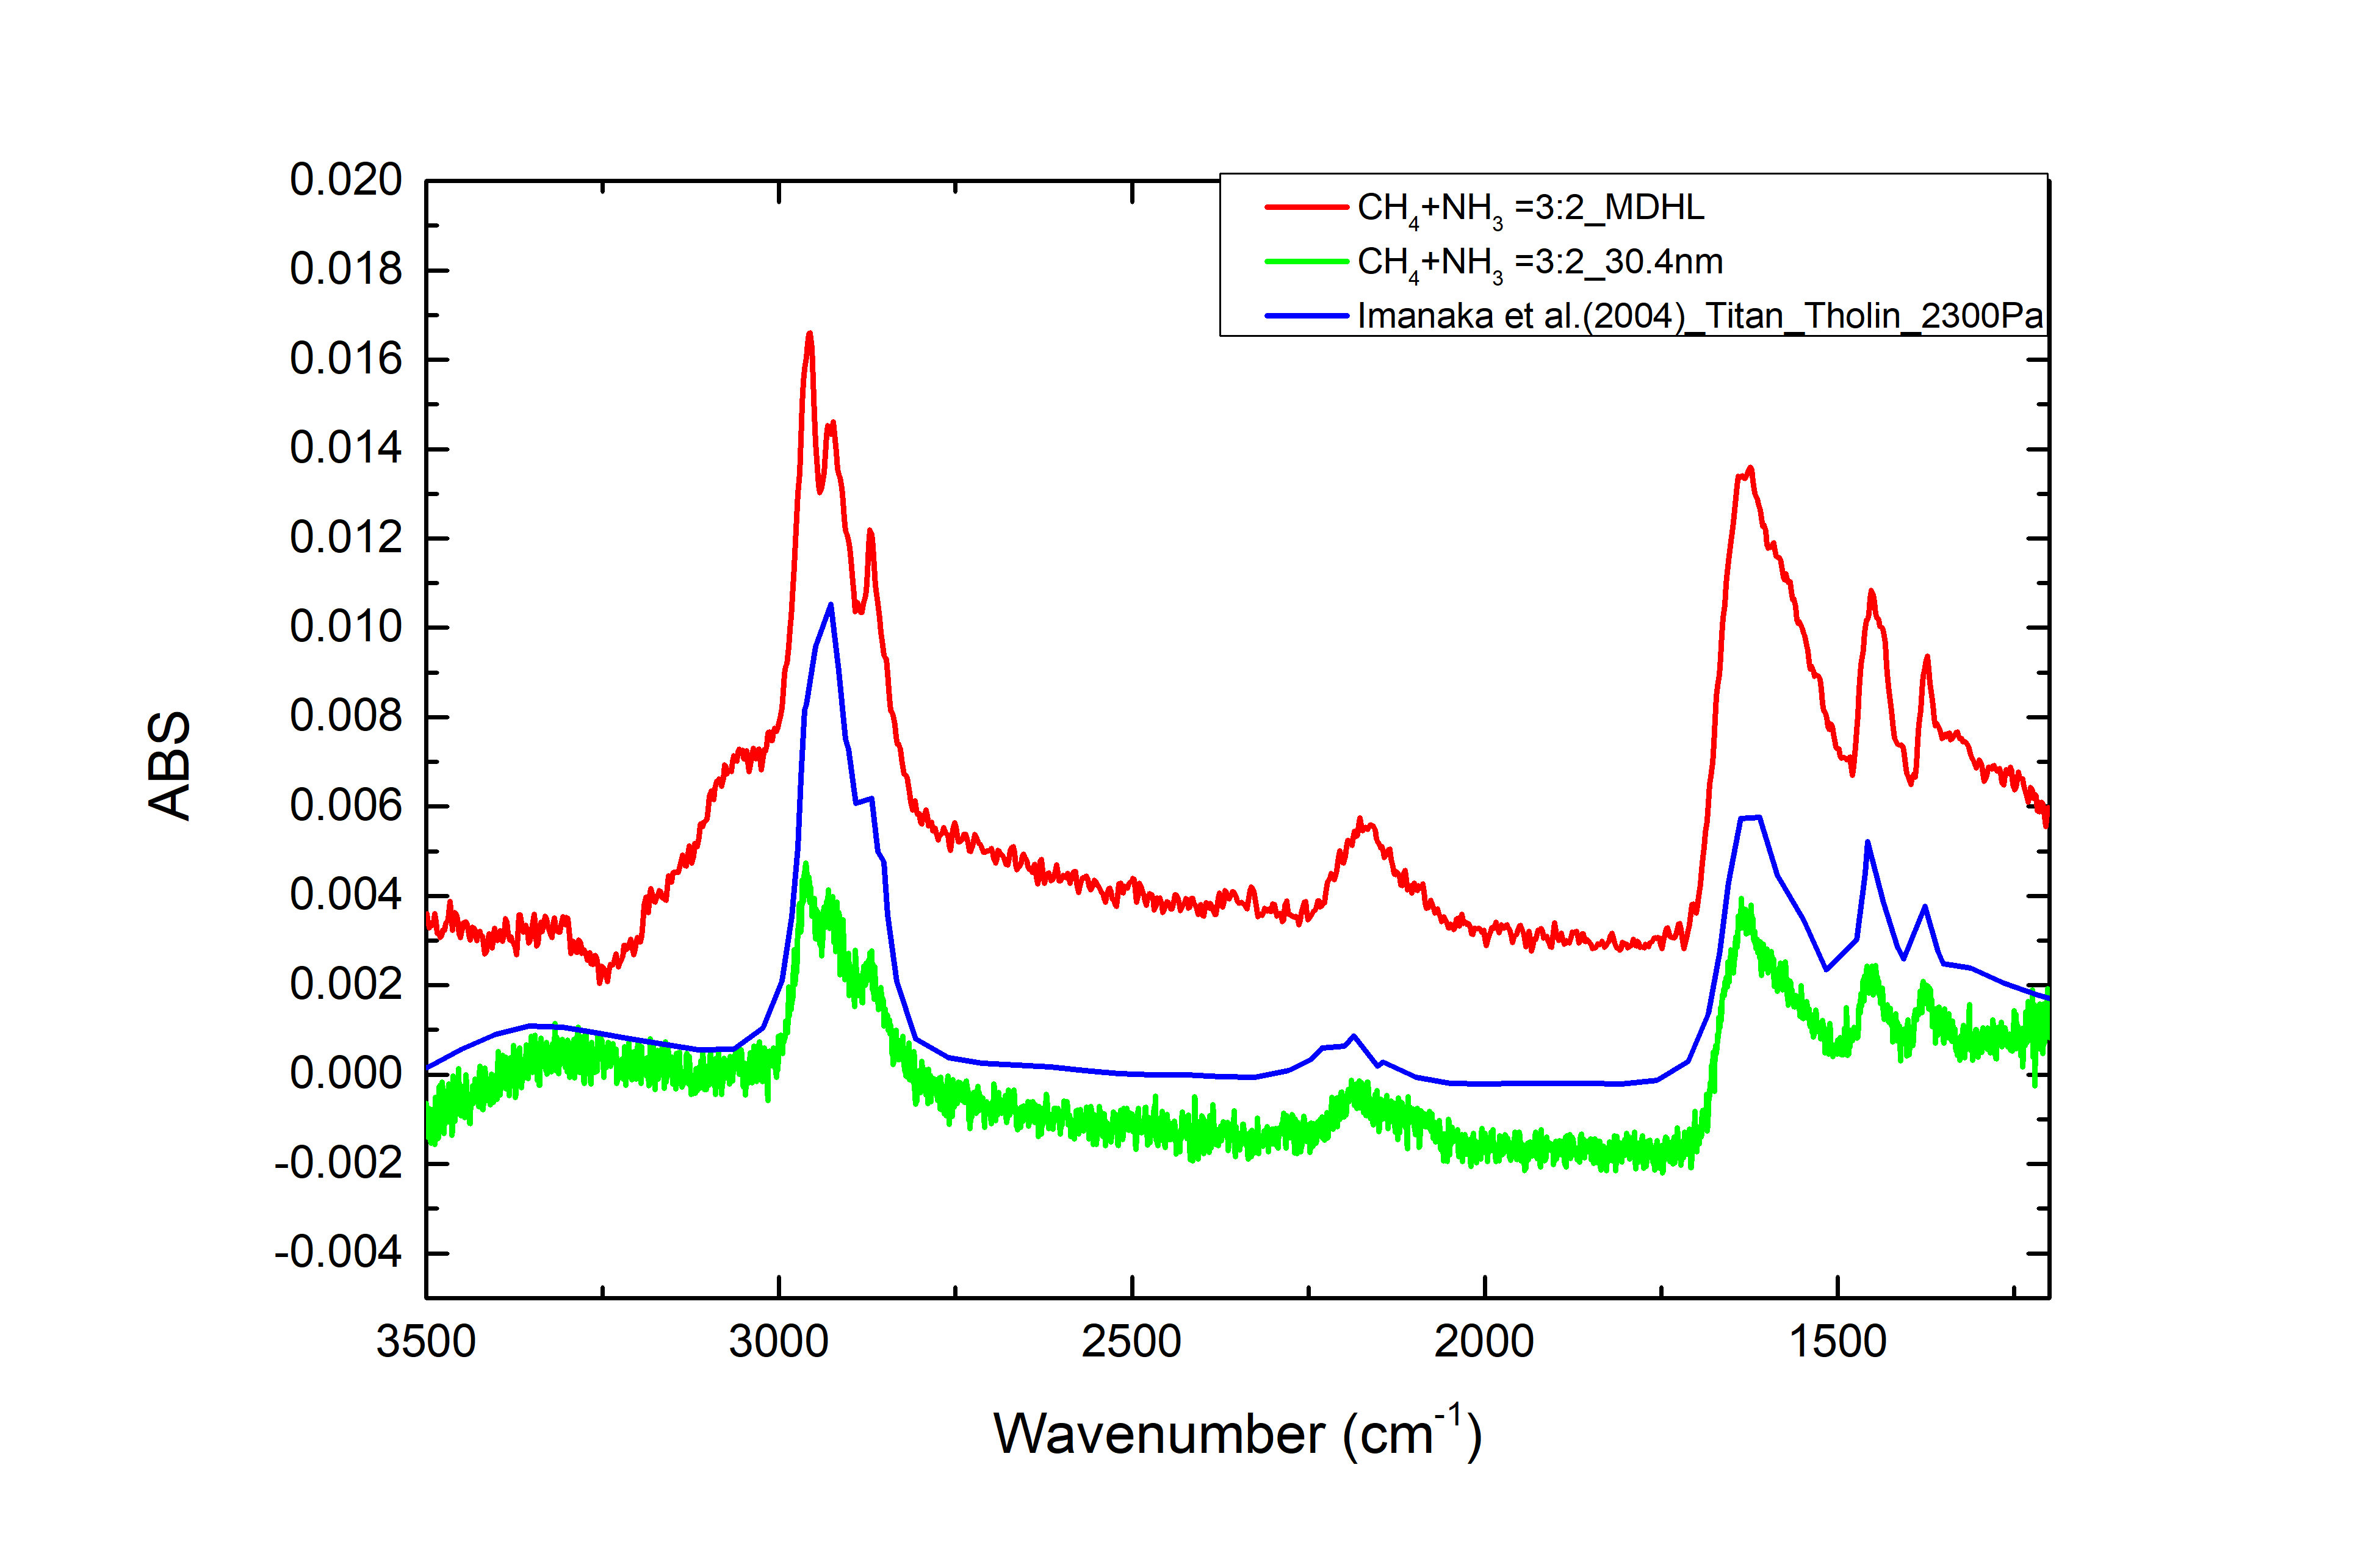
\includegraphics[width=\textwidth]{figures/chapter3/residues.png}
\caption{The IR spectrum of residues in after CH$_4$:NH$_3$ = 3:2 experiments and the accumulate residues after MDHL experiments and NSRRC experiments.}
\label{fig:residues}
\end{figure}


\section{Summary} % should be in chapter 4?

The main product of VUV and EUV irradiated CH$_4$+NH$_3$ ice mixtures are C$_2$H$_6$ and CN$^-$. C$_3$H$_8$ is also produced by C$_2$H$_6$ or C$_2$H$_2$. We do several investigations towards CH$_4$+NH$_3$ ice mixtures. First, by changing ratio of CH$_4$ to NH$_3$ ice mixtures, CN$^-$ production is more effective in NH$_3$ dominated ice mixtures. While in contrast, C$_2$H$_6$ is the main product when CH$_4$ dominates. Second, by changing the photon source to EUV irradiation, the yield of C$_3$H$_8$ increases. By studying the production efficiencies, the difference in photo-production yield is mainly caused by the decrease in photo-destruction cross-section in the reactants. Finally, we compare our residues obtained with laboratory produced Taitan tholins, the similar infrared spectrum shows a similar functional groups in residues. Our result implies that the tholin on Charon should be similar to that of Titan.


